\documentclass[journal]{Setup/IEEEtran}

% *** MISC UTILITY PACKAGES ***
%
%\usepackage{ifpdf}
% Heiko Oberdiek's ifpdf.sty is very useful if you need conditional
% compilation based on whether the output is pdf or dvi.
% usage:
% \ifpdf
%   % pdf code
% \else
%   % dvi code
% \fi
% The latest version of ifpdf.sty can be obtained from:
% http://www.ctan.org/tex-archive/macros/latex/contrib/oberdiek/
% Also, note that IEEEtran.cls V1.7 and later provides a builtin
% \ifCLASSINFOpdf conditional that works the same way.
% When switching from latex to pdflatex and vice-versa, the compiler may
% have to be run twice to clear warning/error messages.

% *** CITATION PACKAGES ***
%
\usepackage{cite}
% cite.sty was written by Donald Arseneau
% V1.6 and later of IEEEtran pre-defines the format of the cite.sty package
% \cite{} output to follow that of IEEE. Loading the cite package will
% result in citation numbers being automatically sorted and properly
% "compressed/ranged". e.g., [1], [9], [2], [7], [5], [6] without using
% cite.sty will become [1], [2], [5]--[7], [9] using cite.sty. cite.sty's
% \cite will automatically add leading space, if needed. Use cite.sty's
% noadjust option (cite.sty V3.8 and later) if you want to turn this off.
% cite.sty is already installed on most LaTeX systems. Be sure and use
% version 4.0 (2003-05-27) and later if using hyperref.sty. cite.sty does
% not currently provide for hyperlinked citations.
% The latest version can be obtained at:
% http://www.ctan.org/tex-archive/macros/latex/contrib/cite/
% The documentation is contained in the cite.sty file itself.






% *** GRAPHICS RELATED PACKAGES ***
%
\ifCLASSINFOpdf
  \usepackage[pdftex]{graphicx}
  % declare the path(s) where your graphic files are
  \graphicspath{{1_introduction/Figs/}{1_methods/Figs/}{3_results/Figs/}{4_discussion_and_conclusions/Figs/}}
  % and their extensions so you won't have to specify these with
  % every instance of \includegraphics
  \DeclareGraphicsExtensions{.pdf,.jpeg,.png}
\else
  % or other class option (dvipsone, dvipdf, if not using dvips). graphicx
  % will default to the driver specified in the system graphics.cfg if no
  % driver is specified.
  % \usepackage[dvips]{graphicx}
  % declare the path(s) where your graphic files are
  % \graphicspath{{../eps/}}
  % and their extensions so you won't have to specify these with
  % every instance of \includegraphics
  % \DeclareGraphicsExtensions{.eps}
\fi
% graphicx was written by David Carlisle and Sebastian Rahtz. It is
% required if you want graphics, photos, etc. graphicx.sty is already
% installed on most LaTeX systems. The latest version and documentation can
% be obtained at: 
% http://www.ctan.org/tex-archive/macros/latex/required/graphics/
% Another good source of documentation is "Using Imported Graphics in
% LaTeX2e" by Keith Reckdahl which can be found as epslatex.ps or
% epslatex.pdf at: http://www.ctan.org/tex-archive/info/
%
% latex, and pdflatex in dvi mode, support graphics in encapsulated
% postscript (.eps) format. pdflatex in pdf mode supports graphics
% in .pdf, .jpeg, .png and .mps (metapost) formats. Users should ensure
% that all non-photo figures use a vector format (.eps, .pdf, .mps) and
% not a bitmapped formats (.jpeg, .png). IEEE frowns on bitmapped formats
% which can result in "jaggedy"/blurry rendering of lines and letters as
% well as large increases in file sizes.
%
% You can find documentation about the pdfTeX application at:
% http://www.tug.org/applications/pdftex





% *** MATH PACKAGES ***
%
\usepackage[cmex10]{amsmath}
\usepackage{amsfonts}

% A popular package from the American Mathematical Society that provides
% many useful and powerful commands for dealing with mathematics. If using
% it, be sure to load this package with the cmex10 option to ensure that
% only type 1 fonts will utilized at all point sizes. Without this option,
% it is possible that some math symbols, particularly those within
% footnotes, will be rendered in bitmap form which will result in a
% document that can not be IEEE Xplore compliant!
%
% Also, note that the amsmath package sets \interdisplaylinepenalty to 10000
% thus preventing page breaks from occurring within multiline equations. Use:
\interdisplaylinepenalty=2500
% after loading amsmath to restore such page breaks as IEEEtran.cls normally
% does. amsmath.sty is already installed on most LaTeX systems. The latest
% version and documentation can be obtained at:
% http://www.ctan.org/tex-archive/macros/latex/required/amslatex/math/





% *** SPECIALIZED LIST PACKAGES ***
%
%\usepackage{algorithmic}
% algorithmic.sty was written by Peter Williams and Rogerio Brito.
% This package provides an algorithmic environment fo describing algorithms.
% You can use the algorithmic environment in-text or within a figure
% environment to provide for a floating algorithm. Do NOT use the algorithm
% floating environment provided by algorithm.sty (by the same authors) or
% algorithm2e.sty (by Christophe Fiorio) as IEEE does not use dedicated
% algorithm float types and packages that provide these will not provide
% correct IEEE style captions. The latest version and documentation of
% algorithmic.sty can be obtained at:
% http://www.ctan.org/tex-archive/macros/latex/contrib/algorithms/
% There is also a support site at:
% http://algorithms.berlios.de/index.html
% Also of interest may be the (relatively newer and more customizable)
% algorithmicx.sty package by Szasz Janos:
% http://www.ctan.org/tex-archive/macros/latex/contrib/algorithmicx/




% *** ALIGNMENT PACKAGES ***
%
%\usepackage{array}
% Frank Mittelbach's and David Carlisle's array.sty patches and improves
% the standard LaTeX2e array and tabular environments to provide better
% appearance and additional user controls. As the default LaTeX2e table
% generation code is lacking to the point of almost being broken with
% respect to the quality of the end results, all users are strongly
% advised to use an enhanced (at the very least that provided by array.sty)
% set of table tools. array.sty is already installed on most systems. The
% latest version and documentation can be obtained at:
% http://www.ctan.org/tex-archive/macros/latex/required/tools/


%\usepackage{mdwmath}
%\usepackage{mdwtab}
% Also highly recommended is Mark Wooding's extremely powerful MDW tools,
% especially mdwmath.sty and mdwtab.sty which are used to format equations
% and tables, respectively. The MDWtools set is already installed on most
% LaTeX systems. The lastest version and documentation is available at:
% http://www.ctan.org/tex-archive/macros/latex/contrib/mdwtools/


% IEEEtran contains the IEEEeqnarray family of commands that can be used to
% generate multiline equations as well as matrices, tables, etc., of high
% quality.


%\usepackage{eqparbox}
% Also of notable interest is Scott Pakin's eqparbox package for creating
% (automatically sized) equal width boxes - aka "natural width parboxes".
% Available at:
% http://www.ctan.org/tex-archive/macros/latex/contrib/eqparbox/





% *** SUBFIGURE PACKAGES ***
% \usepackage[tight,footnotesize]{subfigure}
% subfigure.sty was written by Steven Douglas Cochran. This package makes it
% easy to put subfigures in your figures. e.g., "Figure 1a and 1b". For IEEE
% work, it is a good idea to load it with the tight package option to reduce
% the amount of white space around the subfigures. subfigure.sty is already
% installed on most LaTeX systems. The latest version and documentation can
% be obtained at:
% http://www.ctan.org/tex-archive/obsolete/macros/latex/contrib/subfigure/
% subfigure.sty has been superceeded by subfig.sty.



% \usepackage[caption=false]{caption}
% \usepackage[font=footnotesize]{subfig}
% subfig.sty, also written by Steven Douglas Cochran, is the modern
% replacement for subfigure.sty. However, subfig.sty requires and
% automatically loads Axel Sommerfeldt's caption.sty which will override
% IEEEtran.cls handling of captions and this will result in nonIEEE style
% figure/table captions. To prevent this problem, be sure and preload
% caption.sty with its "caption=false" package option. This is will preserve
% IEEEtran.cls handing of captions. Version 1.3 (2005/06/28) and later 
% (recommended due to many improvements over 1.2) of subfig.sty supports
% the caption=false option directly:
\usepackage[caption=false,font=footnotesize]{subfig}
%
% The latest version and documentation can be obtained at:
% corollary
% The latest version and documentation of caption.sty can be obtained at:
% http://www.ctan.org/tex-archive/macros/latex/contrib/caption/




% *** FLOAT PACKAGES ***
%
%\usepackage{fixltx2e}
% fixltx2e, the successor to the earlier fix2col.sty, was written by
% Frank Mittelbach and David Carlisle. This package corrects a few problems
% in the LaTeX2e kernel, the most notable of which is that in current
% LaTeX2e releases, the ordering of single and double column floats is not
% guaranteed to be preserved. Thus, an unpatched LaTeX2e can allow a
% single column figure to be placed prior to an earlier double column
% figure. The latest version and documentation can be found at:
% http://www.ctan.org/tex-archive/macros/latex/base/



%\usepackage{stfloats}
% stfloats.sty was written by Sigitas Tolusis. This package gives LaTeX2e
% the ability to do double column floats at the bottom of the page as well
% as the top. (e.g., "\begin{figure*}[!b]" is not normally possible in
% LaTeX2e). It also provides a command:
%\fnbelowfloat
% to enable the placement of footnotes below bottom floats (the standard
% LaTeX2e kernel puts them above bottom floats). This is an invasive package
% which rewrites many portions of the LaTeX2e float routines. It may not work
% with other packages that modify the LaTeX2e float routines. The latest
% version and documentation can be obtained at:
% http://www.ctan.org/tex-archive/macros/latex/contrib/sttools/
% Documentation is contained in the stfloats.sty comments as well as in the
% presfull.pdf file. Do not use the stfloats baselinefloat ability as IEEE
% does not allow \baselineskip to stretch. Authors submitting work to the
% IEEE should note that IEEE rarely uses double column equations and
% that authors should try to avoid such use. Do not be tempted to use the
% cuted.sty or midfloat.sty packages (also by Sigitas Tolusis) as IEEE does
% not format its papers in such ways.


%\ifCLASSOPTIONcaptionsoff
%  \usepackage[nomarkers]{endfloat}
% \let\MYoriglatexcaption\caption
% \renewcommand{\caption}[2][\relax]{\MYoriglatexcaption[#2]{#2}}
%\fi
% endfloat.sty was written by James Darrell McCauley and Jeff Goldberg.
% This package may be useful when used in conjunction with IEEEtran.cls'
% captionsoff option. Some IEEE journals/societies require that submissions
% have lists of figures/tables at the end of the paper and that
% figures/tables without any captions are placed on a page by themselves at
% the end of the document. If needed, the draftcls IEEEtran class option or
% \CLASSINPUTbaselinestretch interface can be used to increase the line
% spacing as well. Be sure and use the nomarkers option of endfloat to
% prevent endfloat from "marking" where the figures would have been placed
% in the text. The two hack lines of code above are a slight modification of
% that suggested by in the endfloat docs (section 8.3.1) to ensure that
% the full captions always appear in the list of figures/tables - even if
% the user used the short optional argument of \caption[]{}.
% IEEE papers do not typically make use of \caption[]'s optional argument,
% so this should not be an issue. A similar trick can be used to disable
% captions of packages such as subfig.sty that lack options to turn off
% the subcaptions:
% For subfig.sty:
% \let\MYorigsubfloat\subfloat
% \renewcommand{\subfloat}[2][\relax]{\MYorigsubfloat[]{#2}}
% For subfigure.sty:
% \let\MYorigsubfigure\subfigure
% \renewcommand{\subfigure}[2][\relax]{\MYorigsubfigure[]{#2}}
% However, the above trick will not work if both optional arguments of
% the \subfloat/subfig command are used. Furthermore, there needs to be a
% description of each subfigure *somewhere* and endfloat does not add
% subfigure captions to its list of figures. Thus, the best approach is to
% avoid the use of subfigure captions (many IEEE journals avoid them anyway)
% and instead reference/explain all the subfigures within the main caption.
% The latest version of endfloat.sty and its documentation can obtained at:
% http://www.ctan.org/tex-archive/macros/latex/contrib/endfloat/
%
% The IEEEtran \ifCLASSOPTIONcaptionsoff conditional can also be used
% later in the document, say, to conditionally put the References on a 
% page by themselves.





% *** PDF, URL AND HYPERLINK PACKAGES ***
%
\usepackage{url}
% url.sty was written by Donald Arseneau. It provides better support for
% handling and breaking URLs. url.sty is already installed on most LaTeX
% systems. The latest version can be obtained at:
% http://www.ctan.org/tex-archive/macros/latex/contrib/misc/
% Read the url.sty source comments for usage information. Basically,
% \url{my_url_here}.

% multiple comma-delimited references in a \ref command
\usepackage{cleveref}



% *** Do not adjust lengths that control margins, column widths, etc. ***
% *** Do not use packages that alter fonts (such as pslatex).         ***
% There should be no need to do such things with IEEEtran.cls V1.6 and later.
% (Unless specifically asked to do so by the journal or conference you plan
% to submit to, of course. )

% correct bad hyphenation here
\hyphenation{op-tical net-works semi-conduc-tor}

\begin{document}
%
% paper title
% can use linebreaks \\ within to get better formatting as desired
\title{Transformational Diffusion Smoothing Registration of High Resolution Rat Histology}
%
%
% author names and IEEE memberships
% note positions of commas and nonbreaking spaces ( ~ ) LaTeX will not break
% a structure at a ~ so this keeps an author's name from being broken across
% two lines.
% use \thanks{} to gain access to the first footnote area
% a separate \thanks must be used for each paragraph as LaTeX2e's \thanks
% was not built to handle multiple paragraphs
%

\author{Michael~Shell,~\IEEEmembership{Member,~IEEE,}
        John~Doe,~\IEEEmembership{Fellow,~OSA,}
        and~Jane~Doe,~\IEEEmembership{Life~Fellow,~IEEE}% <-this % stops a space
\thanks{M. Shell is with the Department
of Electrical and Computer Engineering, Georgia Institute of Technology, Atlanta,
GA, 30332 USA e-mail: (see http://www.michaelshell.org/contact.html).}% <-this % stops a space
\thanks{J. Doe and J. Doe are with Anonymous University.}% <-this % stops a space
\thanks{Manuscript received April 19, 2005; revised January 11, 2007.}}

% note the % following the last \IEEEmembership and also \thanks - 
% these prevent an unwanted space from occurring between the last author name
% and the end of the author line. i.e., if you had this:
% 
% \author{....lastname \thanks{...} \thanks{...} }
%                     ^------------^------------^----Do not want these spaces!
%
% a space would be appended to the last name and could cause every name on that
% line to be shifted left slightly. This is one of those "LaTeX things". For
% instance, "\textbf{A} \textbf{B}" will typeset as "A B" not "AB". To get
% "AB" then you have to do: "\textbf{A}\textbf{B}"
% \thanks is no different in this regard, so shield the last } of each \thanks
% that ends a line with a % and do not let a space in before the next \thanks.
% Spaces after \IEEEmembership other than the last one are OK (and needed) as
% you are supposed to have spaces between the names. For what it is worth,
% this is a minor point as most people would not even notice if the said evil
% space somehow managed to creep in.



% The paper headers
\markboth{Journal of \LaTeX\ Class Files,~Vol.~6, No.~1, January~2007}%
{Shell \MakeLowercase{\textit{et al.}}: Bare Demo of IEEEtran.cls for Journals}
% The only time the second header will appear is for the odd numbered pages
% after the title page when using the twoside option.
% 
% *** Note that you probably will NOT want to include the author's ***
% *** name in the headers of peer review papers.                   ***
% You can use \ifCLASSOPTIONpeerreview for conditional compilation here if
% you desire.




% If you want to put a publisher's ID mark on the page you can do it like
% this:
%\IEEEpubid{0000--0000/00\$00.00~\copyright~2007 IEEE}
% Remember, if you use this you must call \IEEEpubidadjcol in the second
% column for its text to clear the IEEEpubid mark.

% use for special paper notices
%\IEEEspecialpapernotice{(Invited Paper)}

% make the title area
\maketitle

%!TEX root = ../diffusion_paper.tex
\begin{abstract}
Adjacent histological slices can be coregistered accurately and lead to smooth image volumes, owing to their close morphological resemblance and their similar intensity spectra. However, volumes constructed from serial histology registration do not reflect the true 3-dimensional tissue geometry. Registration of histology to a set of coherent reference images yields an authentic geometry on the organ scale, yet the lower resolution and differing modality of the references leads to noisy, jagged volumes on the microstructural scale.

We present in this chapter an algorithm to align neigbouring slices accurately and smoothly without disturbing large scale tissue shape, based on a microscopic model of diffusion. We develop a mathematically sound and general framework of transformational diffusion, based on the Lie theory of continous groups. Using synthetic geometries of cardiac tissue with artificial noise, we demonstrate a robust and precise dispersion of information between slices on a configurable range of scales, recovering volumes which are orders of magnitude smoother and which have maintained faithfully the underlying geometrical signal. We apply the algorithm to the volumes from Chapter~\ref{cha:coregistration_of_high_resolution_rat_histology}, first globally and then again to the region around an epicardial vessel. Previously indiscernible microvasculature and sheet structure becomes patent. Pericardium and epicardial vessel segmentations show that displacement abberations between adjacent slices of the order of 400$\mu$m are reduced by two orders of magnitude. The methods presented here outperform any such method to reconstruct histological volumes based on reference images currently in the literature. Finally, we discuss several interesting applications and refinements that might be made to the algorithm in specific cases, including anisotropic diffusion based on image features or inter-slice transform magnitudes.
\end{abstract}


% Note that keywords are not normally used for peerreview papers.
\begin{IEEEkeywords}
IEEEtran, journal, \LaTeX, paper, template.
\end{IEEEkeywords}

% For peer review papers, you can put extra information on the cover
% page as needed:
% \ifCLASSOPTIONpeerreview
% \begin{center} \bfseries EDICS Category: 3-BBND \end{center}
% \fi
%
% For peerreview papers, this IEEEtran command inserts a page break and
% creates the second title. It will be ignored for other modes.
\IEEEpeerreviewmaketitle

%!TEX root = ../diffusion_paper.tex
\section{Introduction} % (fold)
\label{sec:introduction}
  \IEEEPARstart{A}{ll} 3D histology reconstruction methods are based on the acquisition of individual 2D histology images, whether from scans of the un-cut surface of the embedded tissue (so-called block face imaging) \cite{Sands2005,Sands2006,Rutherford2012}, or as sections \cite{Burton2006,Plank2009}. In the former case, 2D images are intrinsically registered, and so no alignment is necessary. In the latter case, images are brought into alignment either through registration amongst themselves, or to a coherent reference volume. It will be seen that the most recent methods draw together the advantages of both techniques.
  
  In 2002, Hooks et al. \cite{Hooks2002} sectioned a 0.8 x 0.8 x 3.7mm transmural segment of rat left ventricle and recorded an intrinsically registered volume image of cubic-1.56$\mu$m resolution using confocal microscopy. The resulting volume images were more detailed than any that had been seen before. Using similar techniques in 2012, Rutherford et al. \cite{Rutherford2012} produced a 5.6mm$^3$ volume surrounding a rat anterior left ventricular infarct, with cubic-1$\mu$m resolution. Unfortunately, this approach cannot resolve tissue sections much larger than the samples presented, and certainly not an entire heart.
  
  Adjacent whole-organ histological images are, in the main, extremely similar in shape, have an extremely similar colour profile and are obtained at the same spatial resolution. These characteristics together make for highly accurate and reliable coregistration. Starting from the first slice in a dataset, previous approaches have registered each successive slice to its predecessor, thus constructing a coherent volume \cite{Chakravarty2006,Schmitt2006,Cifor2009,Cifor2011}. However, there are several unacceptable characteristics of volumes generated with these techniques. Because each slice is positioned relative to the previous, the displacement due to any single erroneous registration is propagated to every subsequent slice. Furthermore, the volumes suffer from what is known as the `z-shift effect' \cite{Yushkevich2006} or the `banana problem' \cite{Malandain2004,Lyon2012}, stemming from the fact that if a curved banana were sliced evenly and perpendicularly to its length, a volume obtained with a slice-to-slice method would appear straight, having lost the original curvature of the banana. In the case of whole-organ histology, volumes approach maximum pairwise symmetry, bearing, if any, a merely coincidental relation to the large-scale geometry of the sample. Finally in this case, only rigid registration may be used, because if the size or shape of slices were unconstrained, every slice would approximate the dimensions of the first, and the organ would approximate a fleshy cylinder.
  
  Registering slices to a reference volume circumvents the banana problem. Burton et al. \cite{Burton2006} paved the way for this conjunction by providing MRI rabbit cardiac images of 26.4 x 26.4 x 24.4$\mu$m voxel size with 1.1 x 1.1 x 10$\mu$m histology stacks of the same hearts, and exhibited an initial attempt at slice alignment, guided by the MRI data. Since then, an automated pipeline has been developed, applying iterative 2D and 3D optimised deformations to register the stacks into the MRI geometry \cite{Mansoori2007}. Despite some success with this procedure, the slices are ultimately registered to 2D MRI image that does not correspond to the histology, and the unconstrained non-rigid registration that was employed in the final stage led to unrealistic tissue distortions. These problems notwithstanding, the direct registration of histology to MRI is the best way to move towards global shape correctness if no other reference data is available, and is still a common procedure \cite{Alic2011,Osechinskiy2011,Kimm2012}.
  
  Block face images, taken from the surface of the fixated tissue volume before sectioning, provide an intrinsically coherent and precisely corresponding set of reference images. Although suitable for low-resolution alignment  \cite{Palm2010}, the reference images are very different in appearance to the histology, with a much lower spatial resolution, hindering accurate alignment. Even very small imperfections in the final mappings introduces jaggedness that renders volumetric microstructure almost imperceptible. Algorithms have been proposed to smooth out this noise through the more precise and reliable coregistration of adjacent slices, in both a sequential \cite{Yushkevich2006,Chakravarty2008} and simultaneous \cite{Feuerstein2011} manner. However, these methods are highly parameterised, often involving registrations at a number of scales, using only a subset of the image information available, and are often based on essentially subjective segmentations, rather than purely original images. Furthermore, only the nearest two neighbouring slices are used to dampen transformational noise, and therefore only the very highest frequency of noise can ever be reduced. Most recently, high-resolution reference images have been provided through the use of two-photon tomography and microtomy \cite{Huang2009,Ragan2012}.
  
  Yushkevich et al. attempt to correct for the banana effect in serially registered mouse \cite{Yushkevich2006} and human \cite{Adler2012} brain histological volumes. They first perform a rigid-body banana registration to approximate the dimensions of a full brain volume. Clearly, if a transform less constrained than rigid-body were used, then each slice would resemble the size and, depending on the constraint of the transform, the shape of the first reference slice. A prism-like volume would result, entirely unrelated to the true geometry of the organ. They obtain resampled 2D MRI images corresponding to each section via a rigid 3D registration of the MRI to the z-shifted histology. The volume produced from registering each section to these MRI images is jagged, and so the transformation parameters are Gaussian smoothed to recover some of the continuity of the serial volume. This approach goes a long way to combining the global fidelity of anchoring to a reference volume and the local smoothness of adjacent slice registration. Yet smoothness is limited by the level of success of the individual inter-slice registrations; any error or discontinuity in the serial volume will be transduced directly into the final result. In particular, any differential deformation of adjacent slices during sectioning, either affine or curved, could not be resolved by the rigid-body banana registration, and would manifest as disjoints through the tissue in the z-direction. Moreover, they themselves concede that the method entails a great deal of empirical parameterisation and manual intervention, from the slice segmentation, to the graph edge weighting of the adjacent slice selection, to the width of the Gaussian smoothing of the histology-to-MRI transform parameters.
  
  No mention of non-rigid transforms is mentioned in the Yushkevich implementation. But conceivably, non-rigid interslice registrations could be integrated into the pipeline once the MRI correspondence planes had been established, initialised from the terminus of the rigid registrations. In this case, one would be faced with two disagreeable alternatives. On the one hand, a direct registration could be performed from each slice in the cylindrical, non-rigid banana volume to the reference volume. In this case, most of the slices would be so distant in size, shape and position from alignment with the reference slice as to preclude consistent, successful registration. A better solution would apply the Gaussian smoothing to the transforms from the non-rigid, prism-like banana volume to the reference volume. These transforms could be computed by composing the inverse of the transforms from the rigid banana volume to the non-rigid volume with the transforms from the rigid banana volume to the reference volume. Volumes would certainly be smoother than with the rigid smoothing, as adjacent non-rigid differences have been relaxed. Yet inevitable occasional errors and inaccuracies in alignment would still be present, as slices are only given one algorithmic run to align, and it is implausible that the freedoms inherent in the transform of choice exactly correspond to the distortions undergone by the tissue sections.
  
  Chakravarty et al. \cite{Chakravarty2008} first rigidly align sections of whole mouse brain to an associated block face set, then apply a deformation field transformation to each slice, calculated as the mean of the parameters from defomation fields registering it to the two neighbouring slices. While this may go some way to reducing noise from the block face registrations, the maximum distance of information transfer is one slice, and so only the maximum distortion frequency will be damped.
  
  Techniques have been developed to combine monomodal adjacent slice and multimodal reference registrations simultaneously. Palm et al. \cite{Palm2008} expound a `weighted multi-image mutual information metric', optimising the sum of scaled contributions from both cost functions, and Feuerstein et al. \cite{Feuerstein2011} combine two potential energy functions in a Markov random field model to reconstruct a rat kidney. Not only do these methods require extraneous parameterisation and tuning, but in practice, the superposed cost function will form several distinct local minima; rather than reaching an averaged compromise between the reference images, the optimisation will arrive close to one preferred of several single-image minima, depending on the relative weightings and the transform initialisation.
  
  Finally, \cite{Arganda-Carreras2010} offer an interesting and robust approach to combining monomodal and multimodal alignments, using consistent b-spline-based elastic registrations. Multiple iterations of triple-wise registrations gradually share information in the z-direction and result in smoothing through a spectrum of scales. However, the choice of simultaneous registration leads to the same problem of multiple local minima faced by \cite{Palm2008,Feuerstein2011}.
  
  Enter what will be referred to as `transformational diffusion smoothing': a novel technique incorporating the best features from reference-based and slice-to-slice registration methods, and eliminating the weaknesses of both. The last four sections introduce and detail transformational diffusion smoothing in full, in a manner driven by the requirements of the problem at hand. A revision of the theoretical underpinnings of 1-dimensional Brownian motion is followed by some simple simulation of diffusion on a discrete grid. In a similar vein, a mathematical exposition of transformational diffusion is followed by its application upon a simulated geometry with added artificial affine noise.
  
  % \hfill mds
  %  
  % \hfill January 11, 2007
  % 
  
  % needed in second column of first page if using \IEEEpubid
  %\IEEEpubidadjcol

% section introduction (end)

%!TEX root = ../diffusion_paper.tex
\section{Methods} % (fold)
\label{sec:methods}
  \subsection{Image Acquisition} % (fold)
  \label{sub:image_acquisition}
    \begin{figure}[!t]
      \centering
      \subfloat[]{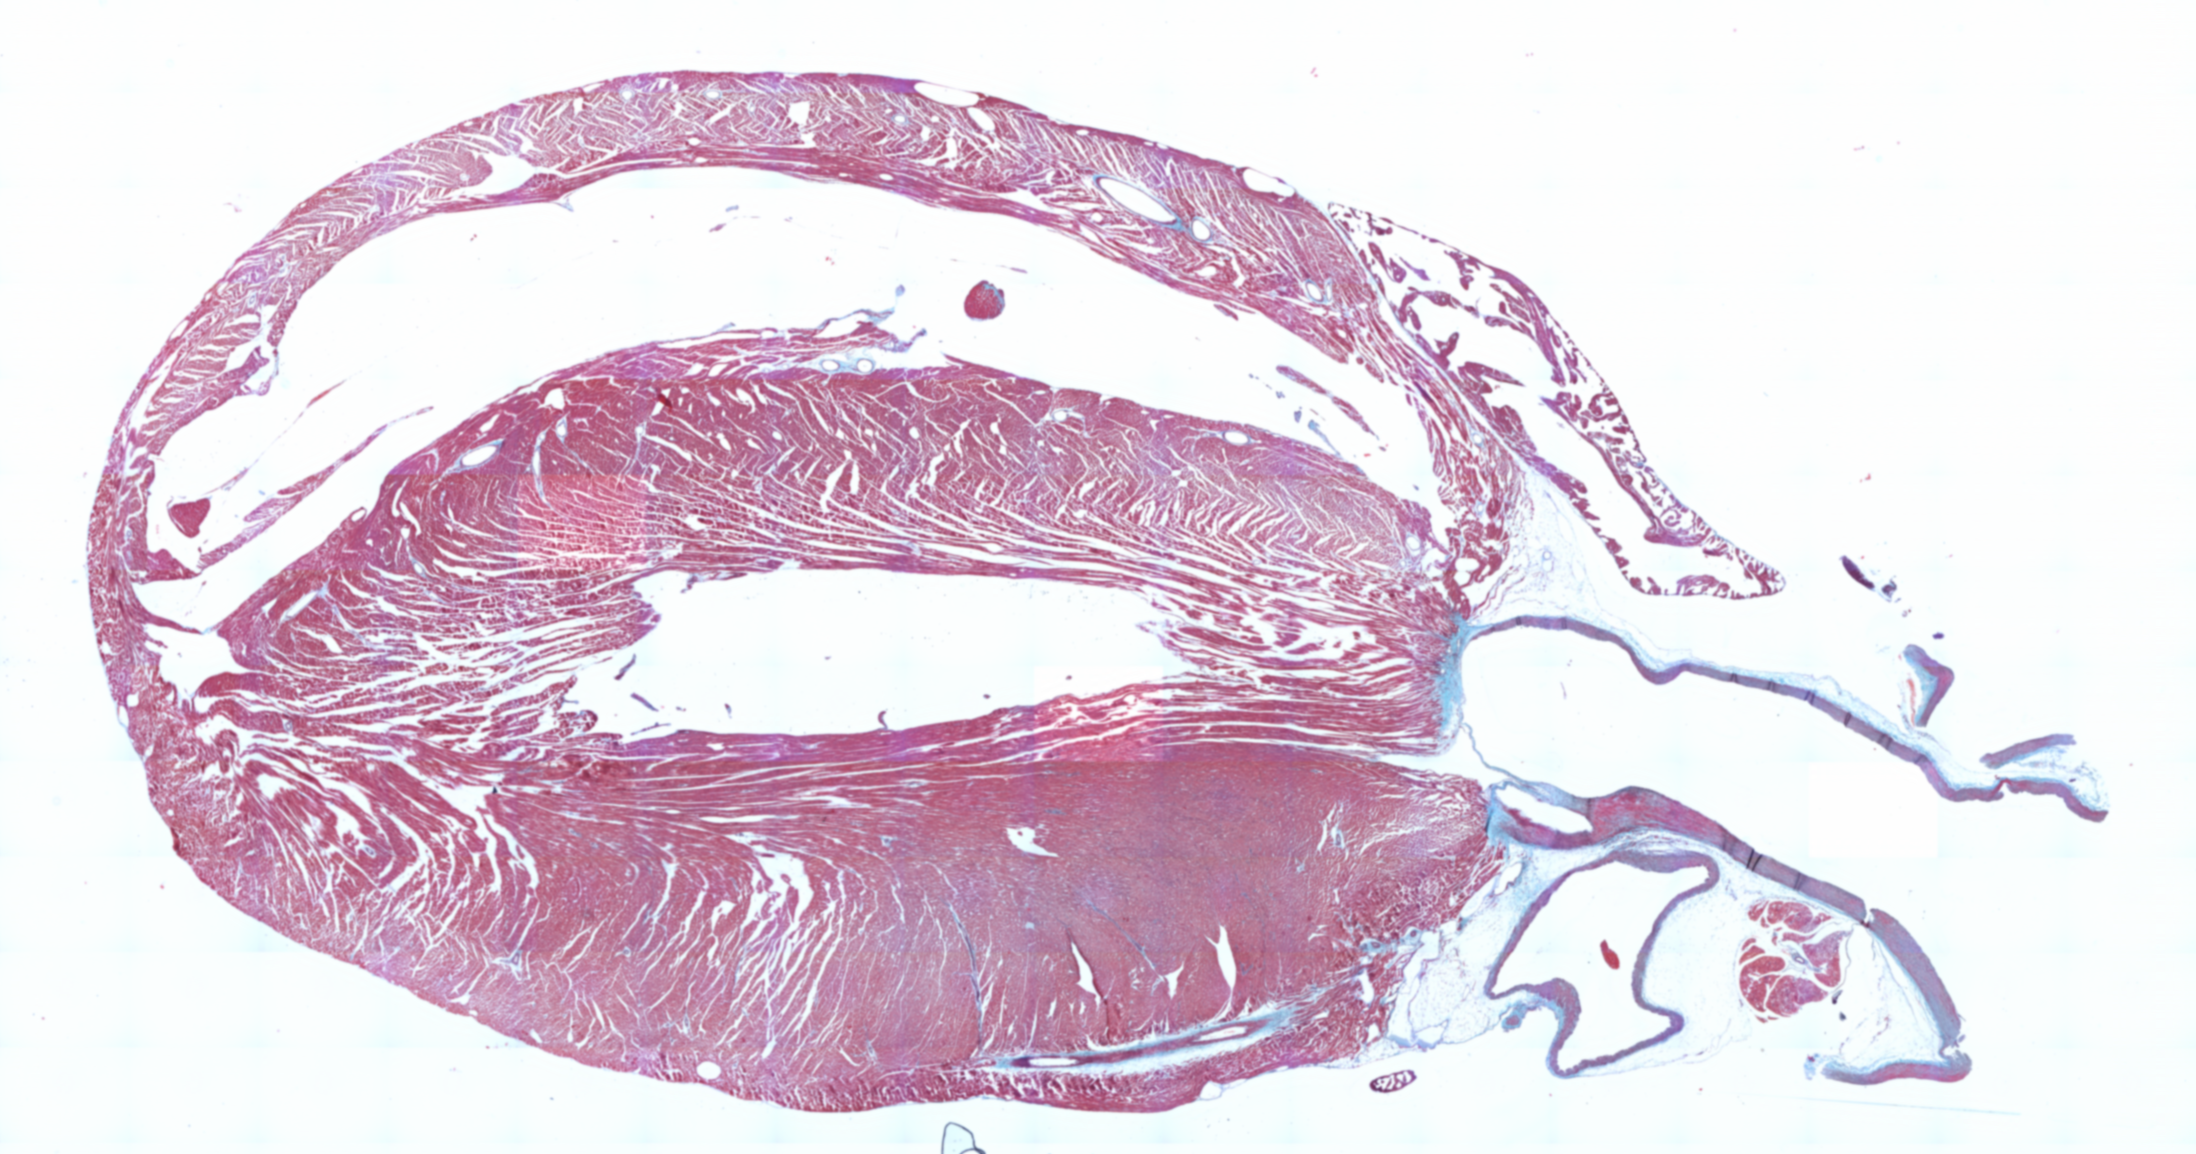
\includegraphics[width=1.7in]{2_methods/Figs/HiRes_downsamples_8_0582}}
      \subfloat[]{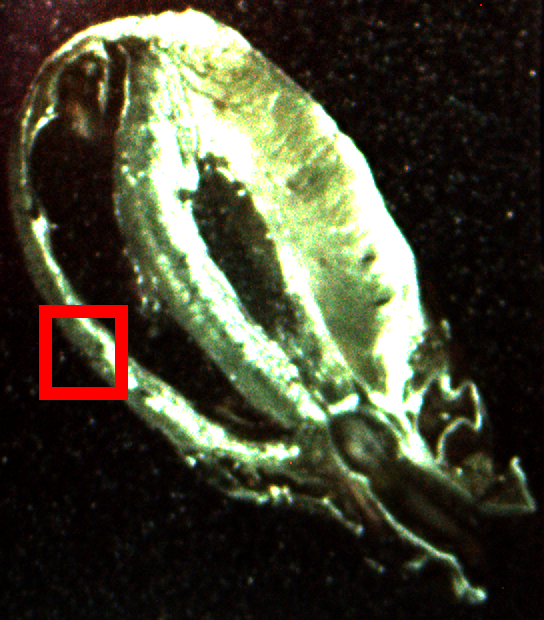
\includegraphics[width=1.7in]{2_methods/Figs/LoRes_rgb_downsamples_1_0582}}\\
      \subfloat[]{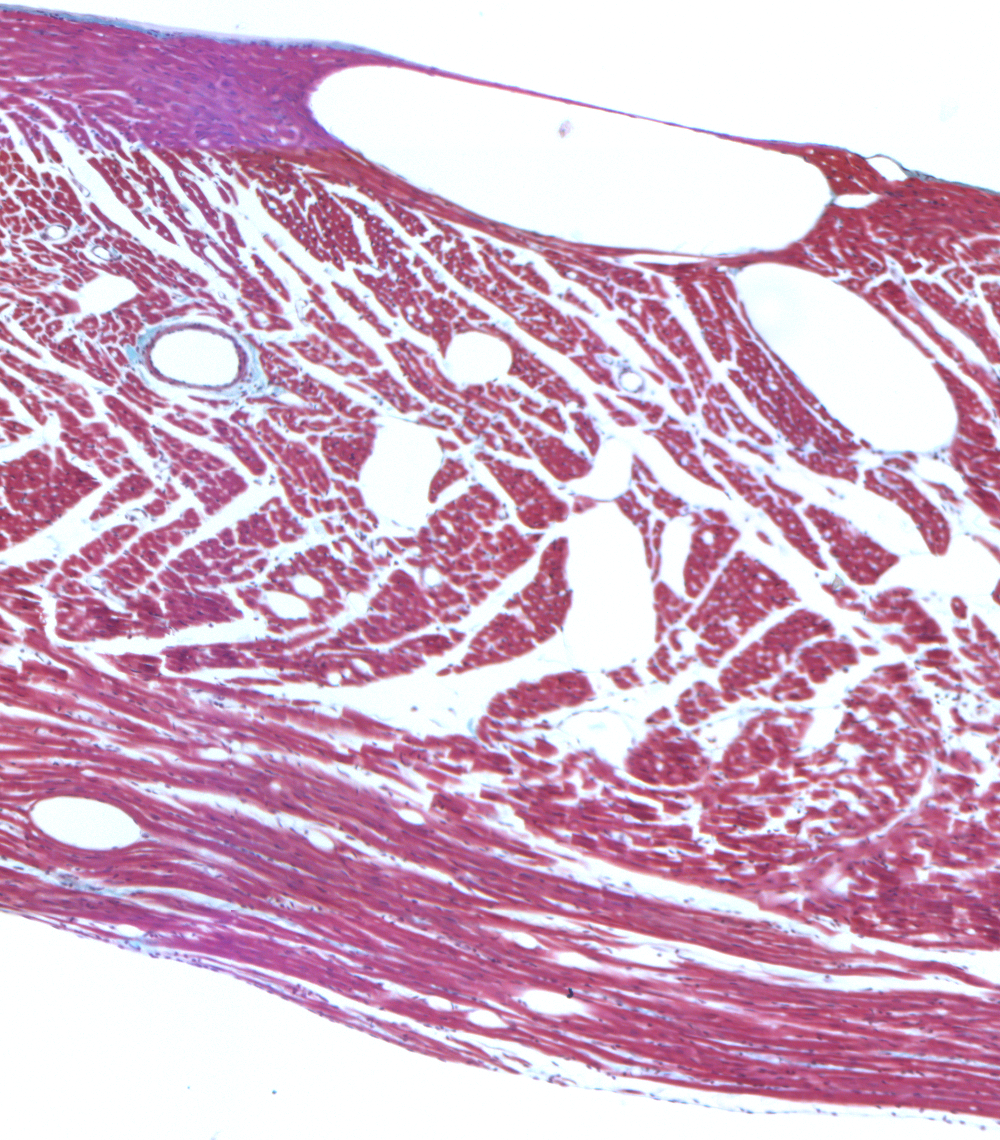
\includegraphics[width=1.7in]{2_methods/Figs/HiRes_downsamples_1_0582_zoom}}
      \subfloat[]{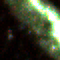
\includegraphics[width=1.7in]{2_methods/Figs/LoRes_rgb_downsamples_1_0582_zoom}}
      \caption{Figure on starting point, showing dataset images, whole and with zoom}
      \label{fig:raw_images}
    \end{figure}

    Hearts were isolated from female rats, fixed and embedded in black wax. The wax blocks were then serially sectioned at 10$\mu$m thickness using a microtome. An image of the top surface of the block -- referred to as a `block face image' from here on -- was taken with 25$\mu$m resolution after each slicing. Each slice was relaxed and rehydrated, before histology imaging was performed using a 5x objective with 1.1$\mu$m resolution, the resultant images being referred to as `histology images' from here on. Gibb et al. \cite{Gibb2012} give a more detailed account of the experimental methods. Examples of the block face and slice images are displayed in Figure~\ref{fig:raw_images}.
  % subsection image_acquisition (end)
  
  \subsection{Block Face Registration} % (fold)
  \label{sub:block_face_registration}
    All registration software developed for the work presented in this paper is based on ITK \cite{Yoo2002} and can be found at \cite{github_registration}. The ITK registration framework consists of the two images to be coregistered, and four main components: a transform, an interpolator, a fitness metric and an optimiser.
    
    Several sets of image downsamples of varying factors were generated, the lowest of which were used for debugging and testing, working up in detail, size and computational expense as the techniques were perfected. The histological images were initialised to their common geometrical centre to create an approximate volume, after which the volume was manually translated to align with the block face volume.
    
    A large proportion of the deformation introduced by the sectioning process is of similarity or affine form. By first registering the simplest of transforms with the lowest dimensional parameter space, and then incrementally relaxing transformational constraint by increasing the number of parameters, we can provide the best possible starting point in each higher dimensional parameter space. Transforms were therefore optimised in the following order, the final result of each initialising its successor: a centered rigid 2D transform - a rotation about an arbitrary centre followed by a translation; a centered similarity transform - as before but with a scaling factor; and a centered affine transform - an affine transformation around an arbitrary centre followed by a translation.

    A mean squares difference metric proved most robust over normalised correlation and mutual information. Parameter scalings were initially chosen based on the dimensions of the images, and subsequently tuned using diagnostic tools that output and visualised transforms and metric values at each iteration of the registration \cite{github_registration}. During registration of a small proportion of the slices, non-monotonicity in the gradient magnitude of the metric along the optimisation path caused the regular step gradient descent optimisation algorithm to reduce its scaling factor prematurely and fail to reach a global optimum. The gradient descent algorithm was therefore employed and yielded more consistent results. A linear interpolator was used to calculate off-grid pixel intensities in all cases.
  % subsection block_face_registration (end)
  
	\subsection{1-Dimensional Brownian Diffusion} % (fold)
	\label{sub:a_1d_random_walk_analogy}
    The central limit theorem states that the mean of a sufficiently large number of independent random variables will be approximately normally distributed, regardless of their individual distribution. Indeed, Einstein's theory of the Brownian motion of a diffusive particle is based on this precept. In particular, the de Moivre-Laplace Theorem states that in the large limit, and in the neighbourhood of the distribution peak, the binomial distribution approximates a Gaussian. In this light, we might consider a concentration of particles $f$ over a discrete 1-dimensional grid $x$, where after a small discretised timestep $\Delta t$, a proportion $2\alpha \Delta t$ of the particles take one step, such that half of them have diffused to the left and half to the right:
	  \begin{equation}
      \begin{split}
  	    f(x_i, t_{n+1}) = f(x_i, t_n) + \alpha (& f(x_{i-1}, t_n) \\
                                                & - 2f(x_i, t_n) \\
                                                & + f(x_{i+1}, t_n)).
      \end{split}
      \label{eqn:diffusion_1d}
		\end{equation}
	  This diffusion will of course act to smooth and homogenise $f$, since regions of high concentration relative to their neighbours will be reduced, and those of low concentration augmented. Since the particles move binomially, in accordance with the de Moivre Laplace Theorem it can be shown that multiple application of this smoothing operation approximates a Gaussian diffusion smoothing.
	% subsection a_1d_random_walk_analogy (end)
	
  \subsection{Transformational Diffusion Smoothing} % (fold)
  \label{sub:transformational_diffusion_smoothing}
    \subsubsection{Algorithm Overview} % (fold)
    \label{ssub:algorithm_overview}
    Our goal is to develop an iterative process that `diffuses' each histological slice image toward its neighbours, in order to smooth out high-frequency transformational noise, whilst maintaining the low-frequency underlying geometry of the volume. A transform $\mathbf{T}$ acting on a point $\mathbf{p}$ maps points in the resampling space to points in the original image space:
  		\begin{equation}
  			\mathbf{p'} = \mathbf{Tp}.
  		\end{equation}
    At iteration $n$ of the proposed process, each slice $i$ in a reconstructed histological stack has associated with it an invertible transform $\mathbf{T}_i^n$. We define the `diffusion transform' $\mathbf{\Delta T}_i^{n,n+1}$, which is formulated to move slice $i$ towards slices $i-1$ and $i+1$, based on the results of registrations between adjacent slices. $\mathbf{\Delta T}_i^{n,n+1}$ is pre-applied to a point in the resampling space of $i$ before $\mathbf{T}_i^n$ to give the adjusted transform $\mathbf{T}_i^{n+1}$, such that
    	\begin{equation}
  			\mathbf{T}_i^{n+1} = \mathbf{T}_i^n \mathbf{\Delta T}_i^{n,n+1}. \label{eqn:adjusted_transforms}
  		\end{equation}
	  It remains to formulate $\mathbf{\Delta T}_i^{n,n+1}$, and this is the subject of the following discussion.
    % subsubsection algorithm_overview (end)
    
    \subsubsection{Formulating the Diffusion Transforms} % (fold)
    \label{ssub:formulating_the_diffusion_transforms}
      In the case of 1-dimensional diffusion, we can reformulate the right hand side of (\ref{eqn:diffusion_1d}) into two separate terms thusly:
	  \begin{alignat}{2}
  	  f(x_i, t_{n+1}) &=\begin{aligned}
        % 1 &+ 2 \\
        % 3 &+ 4
        f(x_i, t_n) + \alpha (&(f(x_{i+1}, t_n) - f(x_i, t_n)) \\
                                    - &(f(x_{i-1}, t_n) - f(x_i, t_n))
  	  \end{aligned} \\
      \Delta f_i^{n,n+1} &= \alpha (\Delta f_{i,i+1}^n - \Delta f_{i-1,i}^n) \\
                         &= \alpha \Delta f_{i,i-1}^n + \alpha \Delta f_{i,i+1}^n, \label{eqn:1d_diffusion_operator}
		\end{alignat}
    where $\Delta f_i^{m,n}$ is the difference in $f$ at position $i$ between timestep $m$ and timestep $n$, and $\Delta f_{i,j}^m$ is the difference in $f$ between position $i$ and position $j$ at timestep $m$. From (\ref{eqn:1d_diffusion_operator}), we can see that at each timestep, the concentration at each bin moves towards its left and right neighbour by a proportion $\alpha$ of its difference from each, respectively.
		
	  We might, then, propose analogously that
		\begin{equation}
		 	\mathbf{\Delta T}_i^{n,n+1} = \alpha \cdot \mathbf{\Delta T}_{i,i+1}^n \oplus \alpha \cdot \mathbf{\Delta T}_{i,i-1}^n, \label{eqn:transformational_placeholder}
		\end{equation}
	 	where $\mathbf{\Delta T}_{i,j}^n = (\mathbf{\Delta T}_{j,i}^n)^{-1}$ is defined as the transformation that registers a histological slice $i$ to slice $j$ at iteration $n$, operator $\cdot$ is a placeholder for a binary operator on a scalar and a transform, and operator $\oplus$ is a placeholder for a binary operator on a pair of transforms. We are now equipped to calculate the transforms for progressively smoother and smoother volumes, by first registering each slice to its neighbour to obtain $\mathbf{\Delta T}_{i,i+1}^n$, then computing the diffusion transforms $\mathbf{\Delta T}_i^{n,n+1}$ through \labelcref{eqn:transformational_placeholder}, and finally applying them to the original transforms through \labelcref{eqn:adjusted_transforms} to obtain $\mathbf{T}_i^{n+1}$. The question now emerges: what precise form do the two binary operators take? We will start by outlining their desirable properties, and then discuss implementations that satisfy these constraints.
    % subsubsection formulating_the_diffusion_transforms (end)
		
    \subsubsection{Formulating the Transform Operators} % (fold)
    \label{ssub:formulating_the_transform_operators}
		The operator $\cdot$ takes two operands: a scalar and a transform. We would like $0$ to be the null operand on $\mathbf{T}$, so that when $\alpha = 0$, no diffusion occurs. We would like $1$ to be the identity operand on $\mathbf{T}$, so that when $\alpha = 1$, the transform from each term in (\ref{eqn:transformational_placeholder}) would diffuse the slice exactly to the position of its equivalent neighbour. Ideally, we would also like addition of the scalar operand to distribute over the serial application of the resultant transforms, so that transforms vary smoothly and naturally with respect to the scalar operand. This final condition can be satisfied for certain transforms, such as linear transforms and vector field transforms, but cannot be satisfied in general for others, such as b-spline transforms. To summarise in mathematical form, we would like the following to hold:
		\begin{gather}
			0 \cdot \mathbf{T} = \mathbf{I} \label{eqn:null} \\
			1 \cdot \mathbf{T} = \mathbf{T} \label{eqn:identity} \\
			(\alpha \cdot \mathbf{T}) (\beta \cdot \mathbf{T}) = (\alpha + \beta) \cdot \mathbf{T} \label{eqn:distributivity}
		\end{gather}
	 	
	  The operator $\oplus$ takes two transform operands. Commutativity must hold if the diffusion is to be symmetric i.e. behave identically if the order of the slices is reversed. If statistics are to be calculated on more than two transformations, it is also necessary for associativity to hold, so that the order of application of operator $\oplus$ is not preferential to any subset of transform operands. That is,
		\begin{gather}
			\forall \mathbf{S}, \mathbf{T} : \mathbf{S} \oplus \mathbf{T} = \mathbf{T} \oplus \mathbf{S} \label{eqn:commutativity} \\
			\forall \mathbf{S}, \mathbf{T} : (\mathbf{S} \oplus \mathbf{T}) \oplus \mathbf{U} = \mathbf{S} \oplus (\mathbf{T} \oplus \mathbf{U}). \label{eqn:associativity}
		\end{gather}
		Unfortunately, commutativity rules out the straightforward serial application of transforms. For example, in the general case of matrix multiplication, $AB \ne BA$. One solution is to use the transform that is equivalent to returning the Euclidian midpoint of $\mathbf{Sp}$ and $\mathbf{Tp}$ for all $\mathbf{p}$. However, the result may not always be representable by some types of transform (notably b-spline transforms), and further, it may be dependent on the order that the $\oplus$ operator is applied. In group theoretical terms, two axioms of the group $(\mathbf{T},\oplus)$ are violated: closure and associativity. Aside from anything else, the Euclidian midpoint approach leads in many cases to unnatural results, such as the `bulging' effect noted in \cite{Arsigny2005a}, and the null matrix in 2D between transforms separated by a rotation of $\pi$.
        
	  It is elucidating to consider the general mathematical form constrained by \labelcref{eqn:null,eqn:identity,eqn:distributivity,eqn:commutativity,eqn:distributivity} applied to concrete classes of transform, in order of increasing complexity: translation transforms, rotation transforms, similarity transforms, affine transforms and more general deformable transforms. An affine transform $\mathbf{T}$ acting on a point $\mathbf{p}$ consists of a matrix transformation $\mathbf{M}$, followed by a translation by an offset vector $\mathbf{o}$:
		\begin{equation}
			\mathbf{p'} = \mathbf{Tp}= \mathbf{Mp} + \mathbf{o}.
		\end{equation}
		In the simplest case of translation transforms, where $\mathbf{M}$ is the identity matrix $\mathbf{I}$ i.e. $\mathbf{Tp} = \mathbf{p} + \mathbf{o}$, the two translation parameters are independent and individually identical to the 1-dimensional diffusion in (\ref{eqn:1d_diffusion_operator}). Operator $\cdot$ is a scalar multiplication of each offset parameter, and operator $\oplus$ is the commutative serial application of the transforms (or equivalently, addition of the respective parameters):
		\begin{align}
			(\alpha \cdot \mathbf{T}) \mathbf{p} &= \mathbf{p} + \alpha\mathbf{o} \label{eqn:translation_cdot}\\
			(\mathbf{S} \oplus \mathbf{T}) \mathbf{p} &= \mathbf{STp} \\
			                                          &= \mathbf{p} + \mathbf{o_S} + \mathbf{o_T} \label{eqn:translation_oplus}
		\end{align}
		Clearly, these two operators satisfy \labelcref{eqn:null,eqn:identity,eqn:distributivity,eqn:commutativity,eqn:associativity}. (\ref{eqn:transformational_placeholder}) becomes
		\begin{align}
		 	\mathbf{\Delta T}_i^{n,n+1} \mathbf{p} &= (\alpha \mathbf{\Delta T}_{i,i-1}^n) (\alpha \mathbf{\Delta T}_{i,i+1}^n) \mathbf{p} \\
			\mathbf{p} + \mathbf{o}_i^{n,n+1} &= \mathbf{p} + \alpha \mathbf{o}_{i,i-1}^n + \alpha \mathbf{o}_{i,i+1}^n \\
			\mathbf{o}_i^{n,n+1} &= \alpha (\mathbf{o}_{i,i-1}^n + \mathbf{o}_{i,i+1}^n) 
		\end{align}
		The offsets are therefore trivially analogous to (\ref{eqn:1d_diffusion_operator}).
		
		In the case of rigid transforms, $\mathbf{M}$ is a rotation matrix $\mathbf{R}(\theta)$. In 2 dimensions, rotation matrices commute, and the result of their multiplication is simply a rotation matrix with angle equal to the sum of the operands' angles; in the special case where there are no offsets, then serial application of the transforms is a candidate for operator $\oplus$ according to (\ref{eqn:commutativity}):
		\begin{equation}
			\mathbf{S} \oplus \mathbf{T} = \mathbf{R}(\theta_\mathbf{S})\mathbf{R}(\theta_\mathbf{T}) = \mathbf{R}(\theta_\mathbf{S} + \theta_\mathbf{T}) = \mathbf{T} \oplus \mathbf{S}
		\end{equation}
		In a similar vein, an operator $\cdot$ that multiplies the angle of the input transform with $\alpha$ fulfils criteria \labelcref{eqn:null,eqn:identity,eqn:distributivity}:
    \begin{equation}
      \alpha \cdot \mathbf{T} = \mathbf{R}(\alpha\theta).
    \end{equation}
		
        In the case of similarity transforms with no offset, $\mathbf{M}$ is a rotation matrix $\mathbf{R}$ multiplied by an enlargement $\sigma$:
        \begin{equation}
            \mathbf{T} = \sigma\mathbf{R}(\theta).
        \end{equation}
        Since scalar multiplications commute with matrix transformations, if the operator $\cdot$ is constructed to scale geometrically, the situation is very similar to that of rotation matrices and \labelcref{eqn:null,eqn:identity,eqn:distributivity,eqn:commutativity,eqn:associativity} still apply:
        \begin{gather}
          \alpha \cdot \mathbf{T} = \sigma^{\alpha}\mathbf{R}(\alpha\theta) \\
          \begin{split}
            (\alpha \cdot \mathbf{T})(\beta \cdot \mathbf{T}) &= \sigma^{\alpha + \beta}\mathbf{R}((\alpha + \beta)\theta) \\
                                                              &= (\alpha + \beta) \cdot \mathbf{T}
          \end{split} \\
          \mathbf{S} \oplus \mathbf{T} = \sigma_\mathbf{S}\mathbf{R}(\theta_\mathbf{S})\sigma_\mathbf{T}\mathbf{R}(\theta_\mathbf{T}) = \mathbf{T} \oplus \mathbf{S} \\
          \begin{split}
      			(\mathbf{S} \oplus \mathbf{T}) \oplus \mathbf{U} &= \sigma_\mathbf{S}\sigma_\mathbf{T}\sigma_\mathbf{U}\mathbf{R}(\theta_\mathbf{S} + \theta_\mathbf{T} + \theta_\mathbf{U}) \\
                                                             &= \mathbf{S} \oplus (\mathbf{T} \oplus \mathbf{U}).
          \end{split}
        \end{gather}
		
		In the more general case of diagonalisable affine matrix transformations, in the absence of translations, and when $\mathbf{S}$ and $\mathbf{T}$ can be diagonalised by the same matrix $\mathbf{V}$ i.e. $\mathbf{S} = \mathbf{VD_SV}^{-1}$ and $\mathbf{T} = \mathbf{VD_TV}^{-1}$, commutativity still holds for serial application:
        \begin{equation}
          \begin{split}
      			\mathbf{S} \oplus \mathbf{T} &= \mathbf{ST} \\
                                         &= \mathbf{VD_SV}^{-1}\mathbf{VD_TV}^{-1} \\
                                         &= \mathbf{VD_SD_TV}^{-1} \\
                                         &= \mathbf{VD_TD_SV}^{-1} \\
                                         &= \mathbf{T} \oplus \mathbf{S},
          \end{split}
        \end{equation}
        with associativity of course holding for the serial application of affine transformations in general. However, when $\mathbf{M_S}$ and $\mathbf{M_T}$ no longer commute, serial application of transforms is no longer sufficient. There is also no obvious form of operator $\cdot$ which satisfies \labelcref{eqn:null,eqn:identity,eqn:distributivity}. We must take recourse to a more general formulation of operators $\cdot$ and $\oplus$.
        
        It is here that we must introduce the concept of the matrix exponential:
        \begin{equation}
          e^{\mathbf{M}} = \sum_{k=0}^{\infty}\frac{1}{k!}\mathbf{M}^k. \label{eqn:matrix_exponential}
        \end{equation}
        Conversely, a logarithm $\mathbf{L}$ of a matrix $\mathbf{M}$ is another matrix such that $e^\mathbf{L} = \mathbf{M}$. For any invertible matrix $\mathbf{Y}$, it is clear that
        \begin{gather}
          (\mathbf{YM}\mathbf{Y}^{-1})^n = \mathbf{Y}\mathbf{M}^n\mathbf{Y}^{-1}, n \in \mathbb{N}.
        \end{gather}
        It then follows from (\ref{eqn:matrix_exponential}) that
        \begin{align}
          \mathbf{Y}e^{\mathbf{M}}\mathbf{Y}^{-1} &= \mathbf{Y}\left(\sum_{k=0}^{\infty}\frac{1}{k!}\mathbf{M}^k\right)\mathbf{Y}^{-1} \\
                                                  &= \sum_{k=0}^{\infty}\frac{1}{k!}\mathbf{Y}\mathbf{M}^k\mathbf{Y}^{-1} \\
                                                  &= \sum_{k=0}^{\infty}\frac{1}{k!}(\mathbf{YM}\mathbf{Y}^{-1})^k \label{eqn:diagonal_exp} \\
                                                  &= e^{\mathbf{YM}\mathbf{Y}^{-1}}.
        \end{align}
        If $\mathbf{M}$ is diagonalisable, and we choose a $\mathbf{Y}$ that diagonalises $\mathbf{M}$, such that $\mathbf{D} = \mathbf{YMY}^{-1}$, (\ref{eqn:diagonal_exp}) becomes trivially analogous to the Taylor expansion for a scalar exponential, and we can then simply compute the exponential of each diagonal element of $\mathbf{D}$. It follows that the logarithm of a positive definite diagonal matrix can be computed by taking the logarithm of each of its elements.
        
        It turns out that when a matrix $\mathbf{M}$ has a logarithm $\mathbf{L}$, $\mathbf{M}$ is in a Lie group --- a group on a smooth manifold. $\mathbf{L}$ is the corresponding element of the associated Lie algebra. $\mathbf{L}$ is an `infinitessimal generator', and its value determines the tangent space at the identity $\mathbf{I}$. Informally, this means that there exists a matrix $\mathbf{I} + \epsilon \mathbf{L}$ that is extremely close to the identity, such that when applied repeatedly an extremely large number of times i.e. $(\mathbf{I} + \epsilon \mathbf{L})^n$, the result eventually becomes $\mathbf{M}$.
        
        If we define operator $\cdot$ in terms of the exponential and the logarithm of $\mathbf{M}$, \labelcref{eqn:null,eqn:identity,eqn:distributivity} are all satisfied:
        \begin{gather}
          \alpha \cdot \mathbf{M} = e^{\alpha\ln\mathbf{M}} \\
          0 \cdot \mathbf{M} = e^0 = \mathbf{I} \\
          1 \cdot \mathbf{M} = e^{\ln\mathbf{M}} = \mathbf{M} \\
          \begin{split}
            (\alpha \cdot \mathbf{M})(\beta \cdot \mathbf{M}) &= e^{\alpha\ln\mathbf{M}}e^{\beta\ln\mathbf{M}} \\
                                                              &= e^{(\alpha + \beta)\ln\mathbf{M}} \\
                                                              &= (\alpha + \beta) \cdot \mathbf{M}.
          \end{split}
        \end{gather}
        We can define operator $\oplus$ as a simple addition of the matrix logarithms in log-Euclidian space, followed by a mapping back to transform space with the exponential operator:
        \begin{equation}
          \mathbf{M_S} \oplus \mathbf{M_T} = e^{\ln\mathbf{M_S} + \ln\mathbf{M_T}}.
        \end{equation}
        Because all operations are homomorphic with Euclidian vector space, this operator always fulfils the commutativity and associativity criteria
        \begin{gather}
          \mathbf{M_S} \oplus \mathbf{M_T} = e^{\ln\mathbf{M_S} + \ln\mathbf{M_T}} = \mathbf{M_T} \oplus \mathbf{M_S} \\
          \begin{split}
            (\mathbf{M_S}\oplus\mathbf{M_T})\oplus\mathbf{M_U} &= e^{\ln\mathbf{M_S} + \ln\mathbf{M_T} + \ln\mathbf{M_U}} \\
                                                               &= \mathbf{M_S}\oplus(\mathbf{M_T}\oplus\mathbf{M_U}).
          \end{split}
        \end{gather}
        It is pleasing to note that this new formula coincides with the special cases of rotation, similarity and diagonalisability discussed previously, since whenever the two matrices commute,
        \begin{equation}
          \begin{split}
            \mathbf{M_SM_T} &= e^{\ln\mathbf{M_S}}e^{\ln\mathbf{M_T}} \\
                            &= e^{\ln\mathbf{M_S} + \ln\mathbf{M_T}} \\
                            &= \mathbf{M_S} \oplus \mathbf{M_T}.
          \end{split}
        \end{equation}
        This `log-Euclidian' approach is expounded with Titanic mathematical rigour in \cite{Arsigny2005}. However, being motivated by the interpolation of MRI data, the treatise is limited to tensors; that is, symmetric matrices with no translation.
        
		    So far, the discussion has been limited to cases with zero offset. When offsets are introduced, even when their respective matrices commute, the commutativity of transforms in (\ref{eqn:commutativity}) no longer holds when serial action akin to (\ref{eqn:translation_oplus}) is introduced na\"ively:
        \begin{equation}
          (\mathbf{S} \oplus \mathbf{T})\mathbf{p} = (\mathbf{M_S} \oplus \mathbf{M_T})\mathbf{p} + \mathbf{M_So_T} + \mathbf{o_S} \ne (\mathbf{T} \oplus \mathbf{S})\mathbf{p}.
        \end{equation}
        If commutivity is forced, by averaging the offset contributions from both permutations of the operands i.e.
        \begin{equation}
          \begin{split}
            (\mathbf{S} \oplus \mathbf{T})\mathbf{p} &= (\mathbf{T} \oplus \mathbf{S})\mathbf{p} \\
                                                     &= (\mathbf{M_S} \oplus \mathbf{M_T})\mathbf{p} \\
                                                     &\qquad + \frac{1}{2}\left(\left( \mathbf{M_S} + \mathbf{I} \right) \mathbf{o_T} + \left( \mathbf{M_T} + \mathbf{I} \right)\mathbf{o_S}\right),
          \end{split}
        \end{equation}
        then associativity breaks down. The same underlying structure precludes a linear interpolation in operator $\cdot$ akin to \labelcref{eqn:translation_cdot} in the presence of a non-identical matrix:
        \begin{gather}
          (\alpha \cdot \mathbf{T})(\beta \cdot \mathbf{T})\mathbf{p} = \mathbf{M}_{\alpha+\beta}\mathbf{p} + \beta\mathbf{M}_{\alpha}\mathbf{o} + \alpha\mathbf{o} \ne (\alpha + \beta) \cdot \mathbf{T}.
        \end{gather}
        When $\mathbf{I} - \mathbf{M}$ is invertible --- that is, when none of the eigenvalues of $\mathbf{M}$ are equal to 1 --- we can express a transform as a matrix transformation about a single invariant centre, with no offset:
        \begin{gather}
          \mathbf{Tp} = \mathbf{Mp} + \mathbf{o} = \mathbf{M}(\mathbf{p}-\mathbf{c}) + \mathbf{c} \\
          \mathbf{o} = (\mathbf{I} - \mathbf{M})\mathbf{c} \\
          \mathbf{c} = (\mathbf{I} - \mathbf{M})^{-1}\mathbf{o}.
        \end{gather}
        We can then reformulate operator $\cdot$ as a log-Euclidian transformation about this invariant centre and satisfy distributivity:
        \begin{gather}
          \alpha \cdot \mathbf{T} = e^{\alpha\ln\mathbf{M}}(p - c) + c \label{eqn:affine_cdot} \\
          \begin{split}
            (\alpha \cdot \mathbf{T})(\beta \cdot \mathbf{T}) &= e^{\alpha\ln\mathbf{M}}((e^{\beta\ln\mathbf{M}}(p - c) + c) - c) + c \\
                                                              &= e^{\alpha\ln\mathbf{M}}(e^{\beta\ln\mathbf{M}}(p - c)) + c \\
                                                              &= e^{(\alpha + \beta)\ln\mathbf{M}}(p - c) + c \\
                                                              &= (\alpha + \beta) \cdot \mathbf{T}.
          \end{split}
        \end{gather}
        With this condition satisfied, $\alpha\cdot\mathbf{T}$ is equivalent to $\mathbf{T}^{\alpha}$.
        
        In order to derive the common centre of the two operands of operator $\oplus$, let us consider the infinitesimal case
        \begin{gather}
          \delta \cdot \mathbf{U} = (\delta \cdot \mathbf{S}) \oplus (\delta \cdot \mathbf{T}) \approx (\delta \cdot \mathbf{S}) (\delta \cdot \mathbf{T}) \\
          \begin{aligned}
            &e^{\delta(\ln \mathbf{M_S} + \ln \mathbf{M_T})}\mathbf{p} \\
            &+ (\mathbf{I} - e^{\delta(\ln \mathbf{M_S} + \ln \mathbf{M_T})})\mathbf{c_U}
          \end{aligned} = \begin{aligned}
              &e^{\delta \ln \mathbf{M_S}}e^{\delta \ln \mathbf{M_T}}\mathbf{p} \\
              &+ e^{\delta \ln \mathbf{M_S}}(\mathbf{I} - e^{\delta \ln \mathbf{T}})\mathbf{c_T} \\
              &+ (\mathbf{I} - e^{\delta \ln \mathbf{M_S}})\mathbf{c_S}. \label{eqn:infinitesimal_oplus}
          \end{aligned}
        \end{gather}
        We can see from the series in (\ref{eqn:matrix_exponential}) that
        \begin{equation}
          e^{\delta \ln \mathbf{M}} = \mathbf{I} + \delta \ln \mathbf{M} + \mathcal{O}((\delta \ln \mathbf{M})^2).
        \end{equation}
        Applying this to (\ref{eqn:infinitesimal_oplus}), we obtain
        \begin{equation}
          (\ln\mathbf{M_S} + \ln\mathbf{M_T})\mathbf{c_U} = (\ln\mathbf{M_S})\mathbf{c_S} + (\ln\mathbf{M_T})\mathbf{c_T}.
        \end{equation}
        The general form of operator $\oplus$ is then finally
        \begin{gather}
          \mathbf{S} \oplus \mathbf{T} = e^{\ln\mathbf{M_S} + \ln\mathbf{M_T}}(\mathbf{p} - \mathbf{c}) + \mathbf{c}, \nonumber \\
          \mathbf{c} = (\ln\mathbf{M_S} + \ln\mathbf{M_T})^{-1}((\ln\mathbf{M_S})\mathbf{c_S} + (\ln\mathbf{M_T})\mathbf{c_T}). \label{eqn:affine_oplus}
        \end{gather}
        Commutativity is evident by inspection, and associativity is simply demonstrated:
        \begin{gather}
          \begin{split}
            (\mathbf{S} \oplus \mathbf{T}) \oplus \mathbf{U} &= \exp(\ln(e^{\ln\mathbf{M_S} + \ln\mathbf{M_T}}) + \ln\mathbf{M_U})(\mathbf{p} - \mathbf{c}) \\
                                                             &\quad + \mathbf{c} \\
                                                             &= e^{\ln\mathbf{M_S} + \ln\mathbf{M_T} + \ln\mathbf{M_U}}(\mathbf{p} - \mathbf{c}) + \mathbf{c},
          \end{split} \\
          \begin{split}
            \mathbf{c} =& (\ln\mathbf{M_{S \oplus T}} + \ln\mathbf{M_U})^{-1} \\
                       &\quad ((\ln\mathbf{M_{S \oplus T}})\mathbf{c_{S \oplus T}} + (\ln\mathbf{M_U})\mathbf{c_U}) \\
                       =& (\ln\mathbf{M_S} + \ln\mathbf{M_T} + \ln\mathbf{M_U})^{-1} \\
                       &\quad ((\ln\mathbf{M_S})\mathbf{c_S} + (\ln\mathbf{M_T})\mathbf{c_T} + (\ln\mathbf{M_U})\mathbf{c_U}).
          \end{split}
        \end{gather}
        As a last algebraic-structural perk, it can be shown from \labelcref{eqn:affine_cdot,eqn:affine_oplus} that the operation of $\cdot$ by a scalar distributes over the operation of $\oplus$ on two affine transformations. In particular,
        \begin{equation}
          (\alpha \cdot \mathbf{S}) \oplus (\alpha \cdot \mathbf{T}) = \alpha \cdot (\mathbf{S} \oplus \mathbf{T}).
        \end{equation}
        
        In the case where $\mathbf{M} - \mathbf{I}$ is singular and there is no central invariate coordinate along the singular dimensions, it is of course natural that operator $\cdot$ interpolates the translation coordinates linearly along those dimensions as in (\ref{eqn:translation_cdot}), and that operator $\oplus$ sums translations arithmetically as in (\ref{eqn:translation_oplus}).
        
        A similar Lie theoretical approach must be taken when implementing operators $\cdot$ and $\oplus$ for more general non-rigid transforms, such as displacement field transforms. However, any differentiable transform will approximate an affine transformation at scales smaller than its curvature, and the implementations expounded here will suffice to smooth out those smaller subregions.
    % subsubsection formulating_the_transform_operators (end)
  % subsection transformational_diffusion_smoothing (end)
	
  \subsection{TDS on Synthetic Geometries} % (fold)
    \label{sub:tds_on_synthetic_geometries}
    In order to test the efficacy of the algorithm in a quantitative way, it was necessary to devise several test geometries. A stack of 200 identical histology slices is presented here, incorporating two low-frequency sinusoidal signals: a translational signal of amplitude approximately half the dimension of the heart section, and a rotational signal spanning 90$^{\circ}$, out of phase with the translational signal by by 90$^{\circ}$. The transform parameters of each slice are then perturbed by random Gaussian noise, with translational $\sigma$ equal to half the amplitude of the translational signal, and the affine matrix element $\sigma$ equal to 0.1.
  
  \subsection{TDS on Block Face-Registered Histology} % (fold)
    \label{sub:diffusion_on_block_face_registered_histology}
    20 iterations of TDS were applied to an entire block face-registered rat heart, and a further 20 iterations to a region around a sub-epicardial vessel .The final transforms from the global smoothing were used to initialise the regional smoothing, with the centre of transformation moved to the geometric centre of the region.
% section methods (end)

%!TEX root = ../diffusion_paper.tex
\section{Results} % (fold)
\label{sec:results}
  % figure of full cross-sections, unregistered, banana registered and lo-res registered, with lores equivalent slice
  \begin{figure}[!t]
    \centering
    \subfloat[]{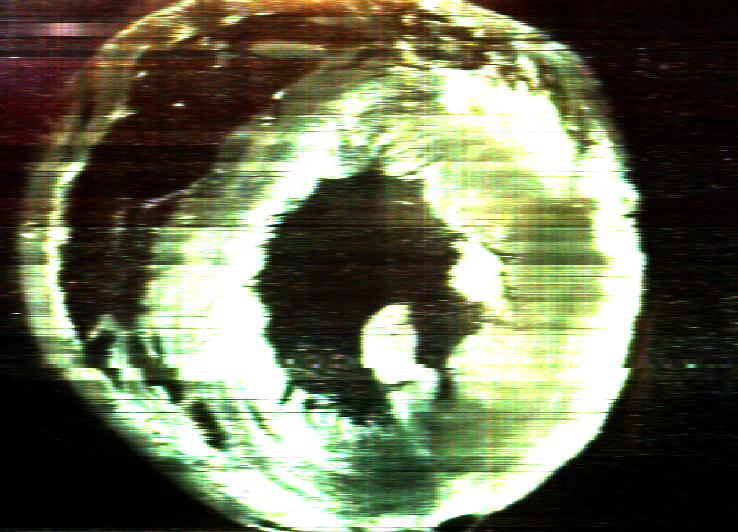
\includegraphics[height=1.2in]{3_results/Figs/LoRes_1_287}}
    \subfloat[]{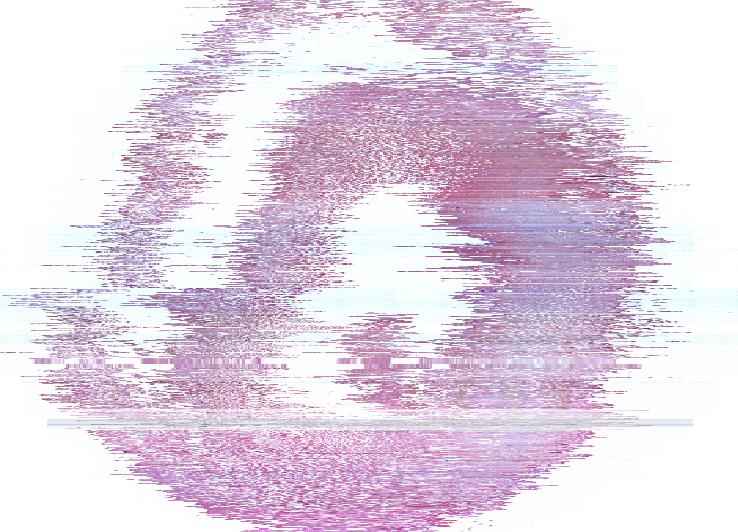
\includegraphics[height=1.2in]{3_results/Figs/geometric_1_287}}\\
    \subfloat[]{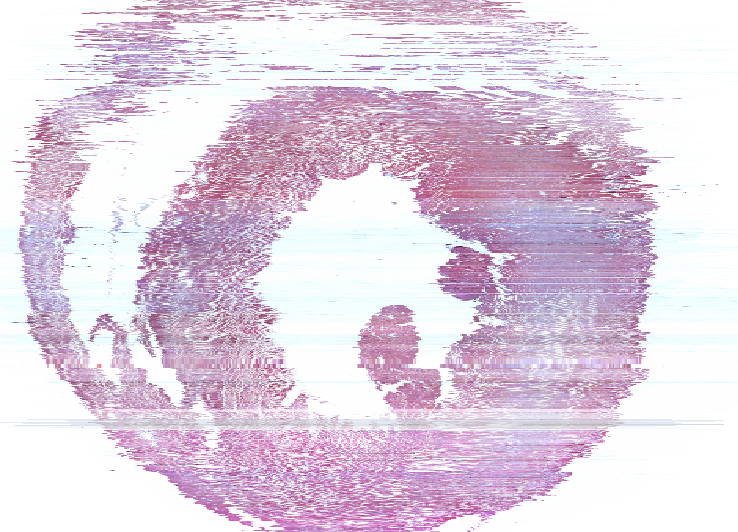
\includegraphics[height=1.2in]{3_results/Figs/affine_1_287}}
    \subfloat[]{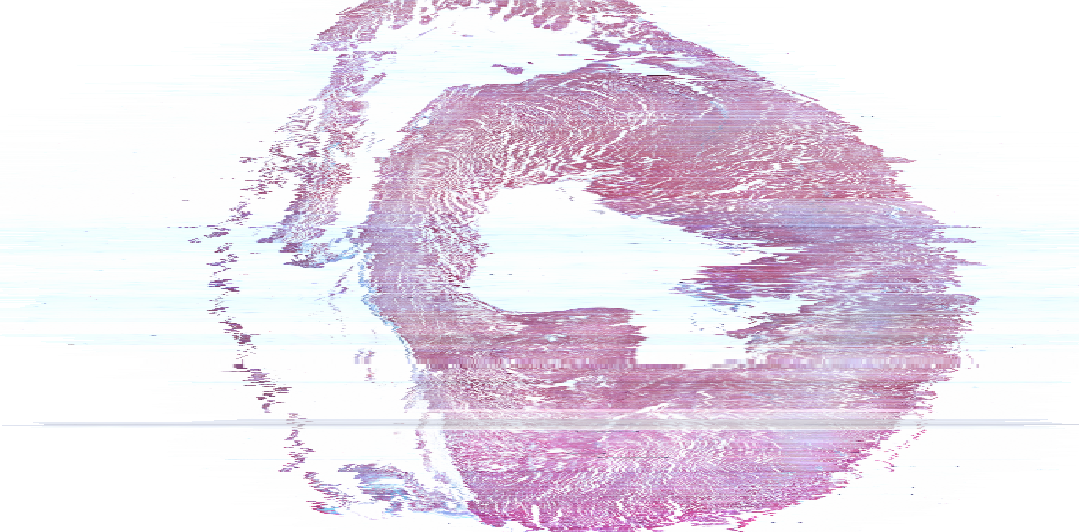
\includegraphics[height=1.2in]{3_results/Figs/banana_1_301}}
    \caption{Equivalent cross-sections of (a) the block face volume, (b) the histology slices before registration, aligned to their common geometrical centre, (c) the block face-registered histology slices and (d) the sequentially registered slices with no reference volume.}
    \label{fig:block_face_registration}
  \end{figure}
  
  Cross-sections of block face, unregistered, block face-registered and serially registered volumes are presented in Figure~\ref{fig:block_face_registration}. We achieve a reasonable large-scale alignment of the great majority of histological slices to form a consistent tissue volume, as is clear from a comparison of Figure~\ref{fig:block_face_registration} (a) and (c). Yet we are left with several limitations of the block face technique. Striations are visible in (a) due to discrete changes in the positioning and intensity of illumination between block face image acquisitions. These changes propagate to the final block face registration result. At 26.6 $\mu$m, the in-plane resolution of the reference images is 24 times coarser than that of the histology slices (evident in Figure~\ref{fig:raw_images}), precluding an alignment on the scale of cardiac microstructure. Small non-rigid deformations introduced during slicing and rehydration are particular to each slice, and could not be represented fully by the affine registration. Despite obtaining a result that was relatively close to the block face geometry, the overlap of pixel intensities between tissue and wax, and the interslice variability therein, leads to a noisy, jagged result that is not always at the global minimum.
  
  Even when constrained by a rigid transform, in many areas the slice-to-slice registration in Figure~\ref{fig:block_face_registration}~(d) is accurate enough that detailed tissue structure is clearly visible. Yet, just as the prism-like synthetic volume does not represent the oscillatory volume in Figure~\ref{fig:synthetic_contours}, the resulting geometry of the volume is quite unrelated to the ground truth of the block face volume.
  
  FROM THESIS
    
  \subsection{Global Diffusion} % (fold)
  \label{sub:global_diffusion}
    % x slices
    \begin{figure}[htbp]
      \caption{Cross-sections of the full Rat28 volume perpendicular to the x-axis, after 0, 1 and 20 iterations of diffusion. The yellow boxes highlight the zoomed regions in Figure~\ref{fig:adjusted_bottom_vessels_0_235}.}
    \end{figure}

    % y slices
    \begin{figure}[htbp]
      \caption{Cross-sections of the full Rat28 volume perpendicular to the y-axis, after 0, 1 and 20 iterations of diffusion. The yellow boxes highlight the zoomed regions in Figure~\ref{fig:adjusted_bottom_vessels_1_287}.}
    \end{figure}
    
    20 iterations of smoothing were applied to the affine registered full-heart volume from Section~\ref{sec:registration_results}, and Figures~\labelcref{fig:adjusted_0_235,fig:adjusted_1_287} compare the central cross-sections of the volume before smoothing, after 1 iteration and after all 20 iterations. A subtle, but unmistakable improvement in coherence is observed; internal and external edges are smoother, especially towards the extremities of the heart, and clear, waving sheet structure has emerged, previously indistinguishable beyond the high-frequency zig-zagging noise.
    
    % lower 100 slices zoom
    % x slices
    \begin{figure}[htbp]
      \caption{Cross-sections of the lower 100 slices perpendicular to the x-axis. The blue arrows highlight blue-stained interstitial tissue around vessels, the green arrow epicardial vessels and the yellow arrow enhanced sheet structure.}
    \end{figure}

    % y slices
    \begin{figure}[htbp]
      \caption{Cross-sections of the lower 100 slices perpendicular to the y-axis. The green arrows highlight epicardial vessels and the yellow arrow enhanced sheet structure.}
    \end{figure}
    
    The effect is clearer in an enlargement of the bottom 100 slices in Figures~\labelcref{fig:adjusted_bottom_vessels_0_235,fig:adjusted_bottom_vessels_1_287}. The outer walls are several orders of magnitude less noisy in both figures, and internal vessel walls are much more coherent, most notably the epicardial vessels on the left and right of Figure~\ref{fig:adjusted_bottom_vessels_1_287}~(c). Sheet structure that started to surface from obscurity after just one iteration has been well resolved after 20 iterations. Figures~\labelcref{fig:whole_positive_x_diffused,fig:whole_negative_x_diffused,fig:whole_positive_y_diffused,fig:whole_positive_z_diffused} depict the smoother global contour after 20 iterations from several angles.
    
    % diffused contours
    \begin{figure}[p]
      \caption{Globally smoothed slice volume, viewed along the positive x direction.}
    \end{figure}

    \begin{figure}[p]
      \caption{Globally smoothed slice volume, viewed along the positive z direction.}
    \end{figure}
  % subsection global_diffusion (end)
  
  % subsection global_diffusion (end)
  
  \subsection{Regional Diffusion} % (fold)
  \label{sub:regional_diffusion}
      \begin{figure}[p]
        \caption{Central cross sections of the region around an epicardial vessel, perpendicular to the x axis. Cross-sections are compared before smoothing, after global smoothing and after smoothing applied to this region. The blue arrow highlights blue-stained interstitial tissue around vessels, the green arrow epicardial vessels and the yellow arrow enhanced sheet structure.}
      \end{figure}
    
      \begin{figure}[p]
        \caption{Central cross sections of the region around an epicardial vessel, perpendicular to the y axis.  The blue arrow highlights blue-stained interstitial tissue around vessels, the green arrow epicardial vessels and the yellow arrow enhanced sheet structure.}
      \end{figure}
    
      % \begin{figure}[p]
      %   \caption{Full resolution image of the central slice of the epicardial vessel region. The yellow box represents the bounds of Figure~\ref{fig:cropped_vessel_cross_section_z}.}
      % \end{figure}
      %     
      % \begin{figure}[p]
      %   \caption{A zoomed 200$\mu$m by 200$\mu$m square of full resolution image of the geometric centre of Figure~\ref{fig:vessel_cross_section_z}.}
      % \end{figure}
    
      A regional registration around an epicardial vessel yields even further improvement, when at this smaller scale, curvature and distortions not represented by an affine transformation become less significant. The final transforms from the global smoothings were used to initialise the regional smoothings, with the centre of transformation moved to the geometric centre of the region. In order to smooth the cost function adequately for the optimiser, the images used to perform the registration were Gaussian smoothed and downsampled by a factor of 8: a level optimal to resolve features the size of an epicardial vessel. Figures~\labelcref{fig:vessel_cross_section_x,fig:vessel_cross_section_y} show two central perpendicular cross-sections of the epicardial region before smoothing, after global smoothing and after an additional regional smoothing. Figures~\labelcref{fig:vessel_cross_section_z,fig:cropped_vessel_cross_section_z} remind us of the order-of-magnitude greater resolution in plane (1.1$\mu$m) with respect to the vertical out-of-plane resolution (10$\mu$m) in Figures~\labelcref{fig:vessel_cross_section_x,fig:vessel_cross_section_y}, displaying the central slice of the region at full resolution.
    
      \begin{figure}[p]
        \caption{Surface contours of segmentations of vasculature (red) and epicardium (green) in the region around an epicardial vessel from Figures~\labelcref{fig:vessel_cross_section_x,fig:vessel_cross_section_y,fig:vessel_cross_section_z,fig:cropped_vessel_cross_section_z}, from the unsmoothed, globally smoothed and locally smoothed volumes.}
      \end{figure}
    
       A confidence connected component segmentation was employed to generate the segmentations in Figure~\ref{fig:region_segmentations}, which, unlike methods such as level set segmentation or neighbourhood filters, does not introduce any artificial surface smoothing. Progressive enhancement in coherence is visible from the back cross-section, the vessel surface and the pericardial surface, from (a) to (b) and then to (c); the contours in (c) are almost totally smooth, with only the inherent stepping of each individual histology slice visible. In particular, the disturbance near the top of the largest vessel in (b) has been smoothed in (c). Original adjacent slice aberrations in (a) reached ~450$\mu$m. Contrastingly in (c), the relative registration error is reduced below the diameter of even the smallest vessels, by inspection less than 5$\mu$m in the large majority of cases - smaller than the width of a single myocyte. Resultingly, with each of the two smoothing procedures, more of the smaller vasculature has become connected to the main vessel and has been segmented.
    
      \begin{figure}[p]
        \caption{An overlay of the three vessel segmentations from Figure~\ref{fig:region_segmentations}. The unsmoothed vessel is shaded in red, the globally smoothed vessel in amber and the regionally smoothed vessel in green. }
      \end{figure}
    
      We see the combined results of all three vascular segmentations in Figure~\ref{fig:vessel_segmentations}. From this view through the pericardium, the striking continuity of the green surface is most apparent. The overall shape of the green vessel precisely intersects the disconnected set of red discs, demonstrating that the underlying vessel geometry has been recovered with remarkable accuracy. Again it is clear that the reduction in error below the diameter of the smallest vessels has facilitated their segmentation, with several thin green dendritic structures reaching up into the top left of the figure.
    
  % subsection regional_diffusion (end)
  
  FROM THESIS

  
  % figure of regional cross-section before smoothing, after global smoothing and after regional smoothing
  \begin{figure}[!t]
    \centering
    \subfloat[]{\includegraphics[width=3.4in]{3_results/Figs/unsmoothed_vessel_1_2125}}\\
    \subfloat[]{\includegraphics[width=3.4in]{3_results/Figs/globally_smoothed_vessel_1_2125}}\\
    \subfloat[]{\includegraphics[width=3.4in]{3_results/Figs/regionally_smoothed_vessel_1_2125}}
    \caption{}
    \label{fig:}
  \end{figure}
  
  % figure of vessel and surface contour before smoothing and after regional smoothing
  \begin{figure}[!t]
    \centering
    \subfloat[]{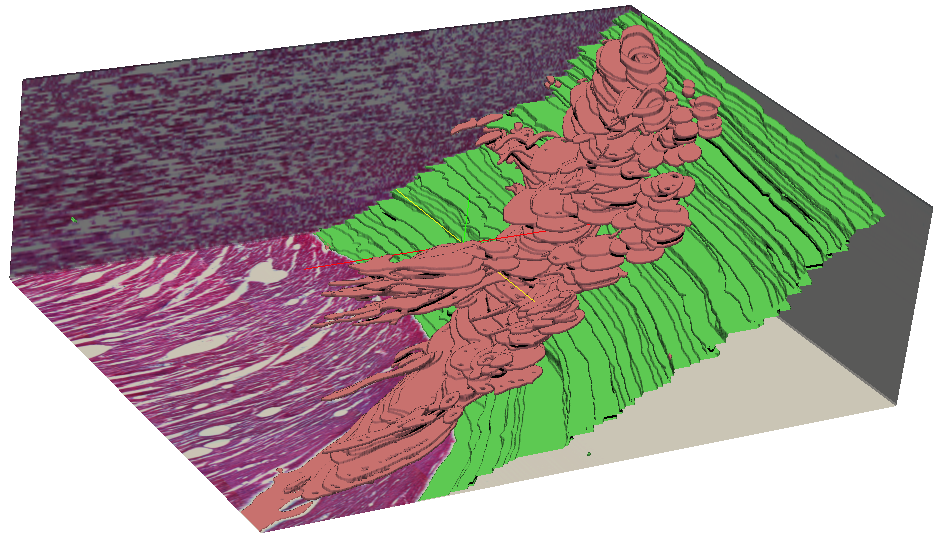
\includegraphics[width=3.4in]{3_results/Figs/unsmoothed_segmentation}}\\
    \subfloat[]{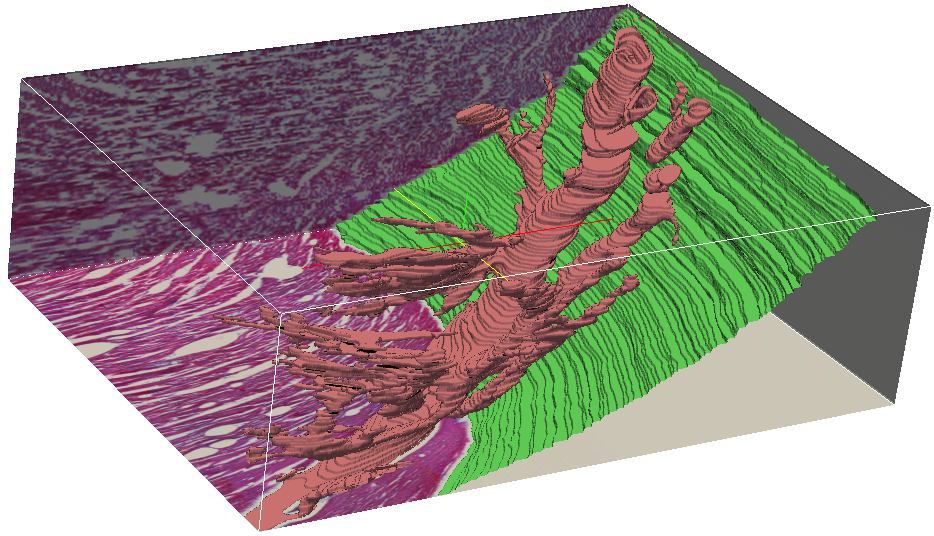
\includegraphics[width=3.4in]{3_results/Figs/globally_smoothed_segmentation}}\\
    \subfloat[]{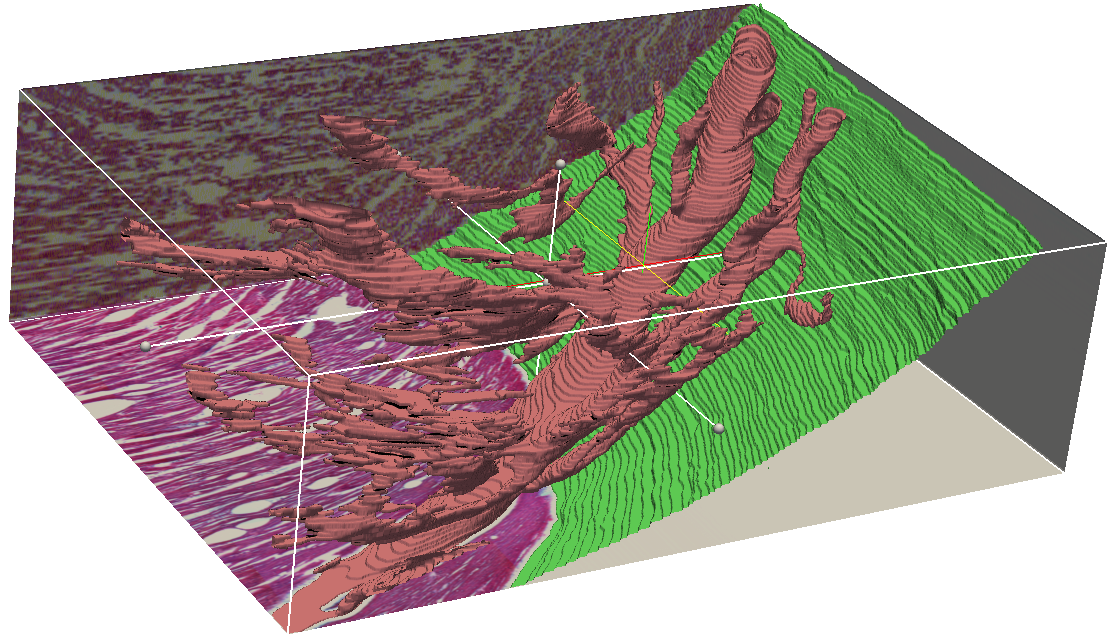
\includegraphics[width=3.4in]{3_results/Figs/locally_smoothed_segmentation}}
    \caption{}
    \label{fig:}
  \end{figure}
  
  % figure of vessel and surface contour before smoothing and after regional smoothing
  \begin{figure}[!t]
    \centering
    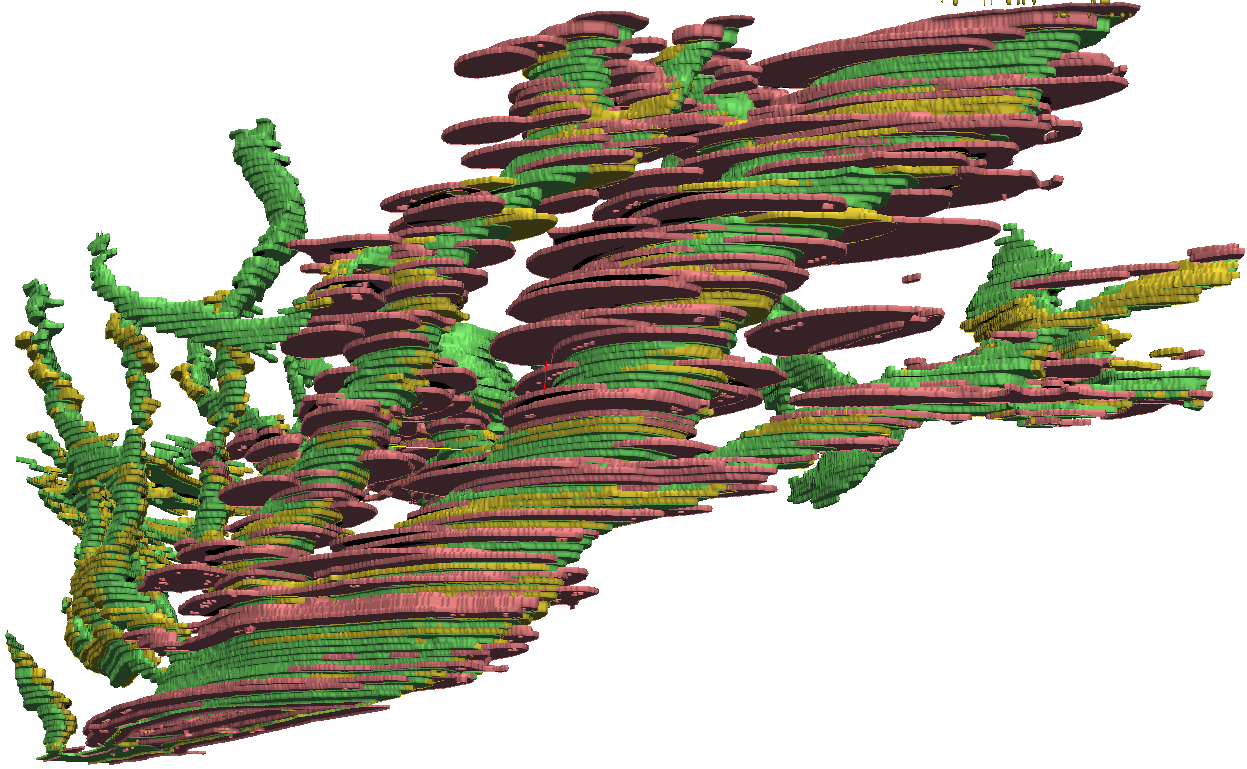
\includegraphics[width=3.4in]{3_results/Figs/vessel_overlay}
    \caption{}
    \label{fig:}
  \end{figure}
% section results (end)

% %!TEX root = ../diffusion_paper.tex
\section{Discussion and Conclusions} % (fold)
\label{sec:discussion_and_conclusions}
  We have invented a robust and mathematically elegant method of resolving volumes from noisy 2-dimensional image slices, transferring transformational information between neighbouring slices. It excels any current technique in the literature at providing smooth, continuous volumes, whilst preserving underlying geometry. Further, its iterative nature confers to it a resilience to the trap of local minima, to registration failures and to outliers, which is unmatched by contemporary methods; even when the cost function of a registration is spiky, and results of a single run are sensitive to initialisation, the TDS algorithm provides multiple opportunities to escape local basins in the cost function, having shifted the cost landscape each time. Contrastingly in the case of banana registration, the displacement from one unsuccessful registration is propagated to \emph{every} subsequent slice in the volume.
  
  One might reasonably consider, as an alternative implementation, the registration of more than just the nearest neighbours at each iteration, but the \emph{k}-nearest neighbours, followed by the application of some (binomial) weighted mean of the results:
  \begin{equation}
    \mathbf{\Delta T}_i^{n,n+1} = \sum_{j=-k}^k \binom{2k}{j+k}\alpha \cdot \mathbf{\Delta T}_{i,i+j}^n,
  \end{equation}
  where we define the sum operator $\sum$ as
  \begin{equation}
    \sum_{i=0}^n \mathbf{T}_i = \mathbf{T}_0 \oplus \mathbf{T}_1 \oplus \ldots \oplus \mathbf{T}_n.
  \end{equation}
  Indeed, in 1-dimensional diffusion, $n$ iterations of nearest neighbour diffusion (where $k=1$) is equivalent to a single binomial iteration across a larger neighbourhood ($k=n$). There are three reasons why this approach is suboptimal. Firstly, inaccurate or erroneous registrations --- most likely to occur in the earliest stages with the most noise --- are given fewer chances to be mitigated by later iterations. Equivalently from another perspective, more registrations are performed under higher levels of perturbation than necessary. Secondly, the further away two histological slices are from each other within the real tissue volume, the more different they appear, and thus a successful registration between them is less likely. Thirdly, no computational time is saved, as the same total number of slice-to-slice registrations must be performed for a given level of smoothing. In fact, total computation is likely to be extended, as the more challenging registrations that are introduced will take longer to reach an optimum.
  
  As was mentioned at the end of Section~\ref{ssub:formulating_the_transform_operators}, this diffusion technique could be extended easily to more complex transforms, as long as that set of transformations form a Lie group. Diffeomorphic transformations fall under this category, and their differentiable and invertible properties are exploited to similar ends in the literature \cite{Avants2006}. Consistent B-splines may also be constrained to be quasi-invertible \cite{Arganda-Carreras2010}. Many transforms commonly used in registration, such as b-spline and other piecewise transforms, are excluded from this classification. In practice, the markedly lax constraint for improvement --- that the algorithm must simply  move each slice somewhat closer to its neighbours --- coupled with the fact that all transforms approximate a Lie group in the small limit, mean that a trivial linear interpolation of any transform's parameters will lead to reliable and geometrically faithful smoothing for noise levels significantly smaller than the scale of the registration.
    
  One of the main decisions when enhancing volumes with TDS is how many iterations should be applied. If the amplitude of the noise frequency spectrum is distributed higher and away from the true underlying geometrical spectrum, then after an initial few iterations of successful noise reduction, the volume will remain largely unchanged in a wide optimal window, whilst a basin of near-zero amplitude frequencies are being damped. Eventually of course, the true low-frequency signal will begin damping, leading to undesired banana-like effects. In practice, it is often simple to detect this window by comparing the output volumes of a range of iteration numbers, looking for the smallest changes in the appearance of cross-sections or segmented contours.
  
  Choosing the optimal number of iterations becomes more complex when preserving genuinely acute image curvature. Just as in the case of 1-dimensional diffusion, true underlying high-frequency signal will be smoothed indiscriminately along with noise. For example, any sharp variation in the cardiac geometry of Section~\ref{sub:regional_diffusion} expressed across fewer than $\sim$5 slices will be smoothed significantly after 20 iterations. Where the banana problem erroneously symmetrises a geometry, TDS can erroneously symmetrise the \emph{curvature} of a geometry, if applied too heavily. Anisotropic TDS based either upon some scalar measure of the magnitude of the transforms between slices, or upon the images or pairs of images themselves, could well be employed to dampen the diffusive coefficient $\alpha$ adaptively, in regions of strong variation where curvature must be preserved. Anisotropic diffusion is used widely in order to clear up noise in the intensity of images, and ~\cite{Arsigny2005} apply anisotropic diffusion to tensor images through a log-Euclidian framework.
  
  Even though the algorithm is robust to the occasional erroneous registration, nothing can make up for a consistent failure to coregister a pair of slices toward each other. In some specific cases, such as a hypothetical straight featureless section of myocardium, the degenerate shapes of slice pairs lead to a flat cost function basin parallel to the myocardial wall, which stifles true matching. Nevertheless, in many cases, careful tuning based on observations of metric value evolution and progress volumes using the tools developed in Section~\ref{sub:diagnostics} can yield a parameter set suitable across all the slice pairs of the volume. Indeed, when registering adjacent slices in the region in Section~\ref{sub:regional_diffusion}, the moving slice pericardium was observed to gravitate quickly and directly towards that of the fixed slice. A slower alignment parallel to the epicardial wall then followed, owing to the displaced but overlapping white epicardial vessel discs, such as in Figure~\ref{fig:vessel_cross_section_z}. In general, image features larger than the maximum amplitude of noise can provide monotonic paths through parameter space to the global minimum.
  
  Boundary conditions at edge slices should be chosen based upon the error in the the edge slice positioning, and upon an estimate of the symmetry at the boundary. Where the error in the edge slice position is thought to be larger than the transformational gradient near the boundary, zero-Neumann discrete boundary conditions can be implemented; a ghost slice that perfectly matches the edge slice with the identity transform is used, along with its single neighbour, to calculate its diffusion at each iteration. This of course introduces banana-like straightening effects near the boundary, as the influx of contributions from the identity penetrate the volume. Alternatively, if the gradient of transformation can be estimated near the boundary, for example via the inverse transforms of the banana registration of the reference images, then non-zero Neumann conditions should be used. Where the positions of boundary slices are considered accurate, Dirichlet-like boundary conditions can lock them in place. Of course, if appropriate, a combination of Neumann and Dirichlet boundary conditions can be implemented.
  
  Going forward, log-Euclidean statistics could be used for averaging pair-wise registrations between 3D data sets, for example between a set of rat hearts. A single representative map could then be developed from the whole dataset, and statistics such as anatomical variation extracted from it. The TDS framework could also be used to smooth out jolting or high-frequency transformational noise in 4D time-series datasets, whilst maintaining the overall positioning of features in space.
  
  Now that we have constructed a smooth, continuous 3D image of cardiac tissue, it remains to extract anatomical information from this volume, with a view to building anatomically-based models for simulation. In the next chapter, we explore the feasibility of such a development.

	MOVE THIS TO DISCUSSION There is a tradeoff to be made when deciding upon a value for the diffusion constant $\alpha$. The greater $\alpha$, the faster and more computationally cheaply the high frequency random noise is damped. But when $\alpha$ approaches 0.5, unstable oscillations start to appear as slices move almost all the way toward the average of their neighbours. In all of the results presented in this paper, $\alpha$ is set to $0.4$. WHAT WE ARE USING IS ESSENTIALLY A FORWARD EULER SCHEME, THERE MIGHT BE OTHER SCHEMES THAT ARE MORE EFFICIENT, BUT THE FACT THAT WE ARE WORKING WITH TRANSFORMS MAKES IT MORE DIFFICULT TO ADAPT THESE SCHEMES TO OUR CASE, AND SO WE HAVEN'T INVESTIGATED THESE SCHEMES FOR THIS PAPER.
% section discussion_and_conclusions (end)


% if have a single appendix:
%\appendix[Proof of the Zonklar Equations]
% or
%\appendix  % for no appendix heading
% do not use \section anymore after \appendix, only \section*
% is possibly needed

% use appendices with more than one appendix
% then use \section to start each appendix
% you must declare a \section before using any
% \subsection or using \label (\appendices by itself
% starts a section numbered zero.)
%


\appendices
\section{Proof of the First Zonklar Equation}
Appendix one text goes here.

% you can choose not to have a title for an appendix
% if you want by leaving the argument blank
\section{}
Appendix two text goes here.


% use section* for acknowledgement
\section*{Acknowledgment}


The authors would like to thank...


% Can use something like this to put references on a page
% by themselves when using endfloat and the captionsoff option.
\ifCLASSOPTIONcaptionsoff
  \newpage
\fi



% trigger a \newpage just before the given reference
% number - used to balance the columns on the last page
% adjust value as needed - may need to be readjusted if
% the document is modified later
%\IEEEtriggeratref{8}
% The "triggered" command can be changed if desired:
%\IEEEtriggercmd{\enlargethispage{-5in}}

% references section

% can use a bibliography generated by BibTeX as a .bbl file
% BibTeX documentation can be easily obtained at:
% http://www.ctan.org/tex-archive/biblio/bibtex/contrib/doc/
% The IEEEtran BibTeX style support page is at:
% http://www.michaelshell.org/tex/ieeetran/bibtex/
\bibliographystyle{IEEEtran}
\bibliography{bibliography}

% biography section
% 
% If you have an EPS/PDF photo (graphicx package needed) extra braces are
% needed around the contents of the optional argument to biography to prevent
% the LaTeX parser from getting confused when it sees the complicated
% \includegraphics command within an optional argument. (You could create
% your own custom macro containing the \includegraphics command to make things
% simpler here.)
%\begin{biography}[{\includegraphics[width=1in,height=1.25in,clip,keepaspectratio]{mshell}}]{Michael Shell}
% or if you just want to reserve a space for a photo:

\begin{IEEEbiography}{Michael Shell}
Biography text here.
\end{IEEEbiography}

% if you will not have a photo at all:
\begin{IEEEbiographynophoto}{John Doe}
Biography text here.
\end{IEEEbiographynophoto}

% insert where needed to balance the two columns on the last page with
% biographies
%\newpage

\begin{IEEEbiographynophoto}{Jane Doe}
Biography text here.
\end{IEEEbiographynophoto}

% You can push biographies down or up by placing
% a \vfill before or after them. The appropriate
% use of \vfill depends on what kind of text is
% on the last page and whether or not the columns
% are being equalized.

%\vfill

% Can be used to pull up biographies so that the bottom of the last one
% is flush with the other column.
%\enlargethispage{-5in}

\end{document}


